%% Royal Society Interface submission
%% Converted from the Elsevier CAS manuscript in paper/els-cas-paper (2026-07-17).
%% Body content is ported VERBATIM from els-cas-paper/main.tex; only the
%% journal wrapping differs (class, front/end matter, biblatex bibliography).
%% Single-column layout: the template's optional \begin{multicols}{2} wrapper
%% is deliberately NOT used.

%% Local-toolchain workaround: this machine's MiKTeX pairs a 2026-06-01 LaTeX
%% kernel with a biblatex that fails to load under it. Rolling the kernel back
%% to 2025-06-01 restores compatibility. Remove once the local MiKTeX is fully
%% updated.
%% The guard is NOT cosmetic. On Overleaf (TeX Live 2025, format 2025-06-01)
%% the unconditional form patches nothing -- "Current format date selected, no
%% patches applied" -- yet still rolls INDIVIDUAL packages back to whatever
%% release best approximates the target: graphics and amsmath both land on
%% their 2019 versions. Loading it only on a format newer than the rollback
%% target confines the workaround to the machine that needs it.
\IfFormatAtLeastTF{2026-01-01}{\RequirePackage[2025-06-01]{latexrelease}}{}

\documentclass[openacc]{rsproca_new}

%% Packages required by the manuscript body (amsmath/amssymb/graphicx/xcolor,
%% hyperref and biblatex are already loaded by the class).
\usepackage{booktabs}
\usepackage{tabularx}
\usepackage{float}
\usepackage{placeins}
\usepackage{enumerate}

%% The supplementary appendix is compiled as a SEPARATE document
%% (appendix.tex -> appendix.pdf). Pull in its labels so that \ref{} to
%% appendix sections/figures/tables resolve to the right numbers.
%% Build order: pdflatex appendix -> pdflatex main -> biber main -> pdflatex main x2.
\usepackage{xr}
\externaldocument{appendix}

%% Bibliography database (style is fixed by the class: biblatex/biber, phys)
\addbibresource{mybib.bib}

%% Numeric subsection numbering (2.1, 3.2, ...) instead of the class default
%% "(a)", "(b)": cross-references such as "Section 3.2" would otherwise print
%% as an ambiguous "(b)", and the standalone supplementary appendix refers to
%% main-text subsections by their numeric form.
\renewcommand\thesubsection{\thesection.\arabic{subsection}}
\renewcommand\thesubsubsection{\thesubsection.\arabic{subsubsection}}

%% Do not stretch vertical glue to force a flush bottom margin: with many
%% large floats this produces big mid-page gaps. Leftover space (if any)
%% goes to the bottom of the page instead.
\raggedbottom

\jname{rsif}
\Journal{J R Soc Interface\ }

\begin{document}

%%%% Article title
\title{Payoff scaling shapes cooperation in LLM agents across languages}

%%%% Authors ($\dagger$: equal contribution, $\star$: corresponding authors)
\author{The Anh Han$^{1,\dagger,\star}$, Trung-Kiet Huynh$^{2,4,\dagger}$, Dao-Sy Duy-Minh$^{2,4,\dagger}$, Thanh-Bang Cao$^{3,4}$, Phong-Hao Le$^{3,4}$, Hong-Dan Nguyen$^{3,4}$, Phu-Quy Nguyen-Lam$^{2,4}$, Minh-Luan Nguyen-Vo$^{3,4}$, Hong-Phat Pham$^{3,4}$, Phu-Hoa Pham$^{2,4}$, Thien-Kim Than$^{3,4}$, Chi-Nguyen Tran$^{3,4}$, Huy Tran$^{3,4}$, Gia-Thoai Tran-Le$^{3,4}$, Alessio Buscemi$^{5}$ and Le Hong Trang$^{3,4,\star}$}

%%%% Author addresses
\address{$^{1}$School of Computing, Engineering and Digital Technologies, Teesside University, Middlesbrough, United Kingdom\\
$^{2}$Faculty of Information Technology, University of Science (HCMUS), Ho Chi Minh City, Vietnam\\
$^{3}$Faculty of Computer Science and Engineering, Ho Chi Minh City University of Technology (HCMUT), Ho Chi Minh City, Vietnam\\
$^{4}$Vietnam National University -- Ho Chi Minh City (VNU-HCM), Ho Chi Minh City, Vietnam\\
$^{5}$Luxembourg Institute of Science and Technology (LIST), Luxembourg\\[4pt]
$^{\dagger}$These authors contributed equally to this work.\\
$^{\star}$Corresponding authors.}

%%%% Subject entries
\subject{artificial intelligence, game theory, multi-agent systems}

%%%% Keyword entries
\keywords{cooperation, large language models, evolutionary game theory, iterated Prisoner's Dilemma, cross-lingual behaviour, intention recognition}

%%%% Corresponding authors
\corres{Le Hong Trang\\
\email{lhtrang@hcmut.edu.vn}\\[2pt]
The Anh Han\\
\email{t.han@tees.ac.uk}}

%%%% Abstract
\begin{abstract}
Large language models (LLMs) are increasingly deployed as autonomous agents that negotiate, coordinate, and act on behalf of users. Whether they cooperate in such settings is no longer just an academic question, but a central issue for AI  governance. We approach it from a strategic-behaviour angle, asking how two everyday levers -- the size of what is at stake, and the language in which the interaction is described -- shape the strategies LLMs adopt in a repeated Prisoner's Dilemma. Rather than reading cooperation off raw action counts, we train supervised classifiers to recognise the canonical strategies of repeated games  (always cooperate, always defect, Tit-for-Tat, Win-Stay--Lose-Shift) and use them as a lens onto LLM behaviour. To know what the strategy distribution \emph{should} look like under the same payoffs, we derive an evolutionary game theory (EGT) baseline and compare it with the LLM data. The two outcomes disagree in a revealing way: as stakes grow, evolutionary theory predicts that defection should take over the population, yet LLMs move in the opposite direction, becoming more cooperative -- a signature, we argue, of alignment training and the human-like reasoning patterns LLMs inherit from their training data. We further show that this picture is not particular to frontier-scale, proprietary models: it also occurs  with three open-weight smaller LLMs. 
Overall, our analysis highlights that payoff design and linguistic framing are powerful but under-explored levers for steering LLM behaviour, with direct implications for evaluating, aligning, and governing multi-agent AI systems deployed in high-stakes, multilingual environments.
\end{abstract}

%% (No \begin{fmtext} first-page block: the long abstract leaves no room on
%% the first page -- the body text would collide with the licence notice.)

\maketitle

\section{Introduction}\label{sec:intro}


Large language models (LLMs) are increasingly deployed as \emph{agents} in recommendation systems, negotiation tools, and multi-agent assistants~\cite{tessler2024ai,hammond2025multi,cook2024llm}. In these settings, LLMs face \emph{cooperation dilemmas} in which behaviour emerges from strategic interactions rather than isolated model outputs. Empirical studies show that such behaviour is shaped by training, prompting, role assignment, and linguistic framing, with direct implications for safety, coordination, and AI governance~\cite{lu2024llms,akata2025,fontana2025nicer,han2026social,idowu2026mapping}. Equally critical is the adaptability of their cooperative strategies to varying costs and benefits (payoff stakes), as this directly influences AI system outcomes across a spectrum of real-world scenarios~\cite{hammond2025multi}.

A growing body of work evaluates LLMs through game-theoretic lenses, particularly via matrix and repeated games, revealing systematic departures from Nash equilibria, persistent cooperative biases, and sensitivity to contextual factors such as language and incentives~\cite{buscemi2025fairgame,akata2025,sun2025gtllm_survey,mao2025alympics,pal2026strategiescooperationdefectionlarge,willis2025will,fan2024can,pires2025large,fu2026optimal}. 
These studies increasingly rely on controlled experimental testbeds that vary models, languages, payoff structures, and agent roles. Yet most existing evaluations still focus on aggregate outcomes---such as cooperation rates or payoff distributions---and do not directly model the \emph{behavioural intentions} underlying observed actions.
%FAIRGAME -- the Framework for AI Agents Bias Recognition using Game Theory~\cite{buscemi2025fairgame} -- provides a controlled experimental testbed for probing these effects across models, languages and personalities. However, most existing evaluations focus on aggregate outcomes, such as cooperation rates or payoff distributions, and do not directly model the \emph{behavioural intentions} underlying observed actions.

Evaluating strategic behaviour at the level required for governance and alignment therefore demands methods that go beyond surface-level outputs. Drawing on behavioural and evolutionary game theory \cite{sigmund:2010bo}, we conceptualise behavioural intention as an agent's \emph{strategy}: a decision rule mapping interaction histories to subsequent actions~\cite{han2011role,diStefanoIntention2023,Han2012ALIFEjournal,fujimoto2019functional}. Classical canonical strategies in repeated games, such as Always Cooperate (ALLC), Always Defect (ALLD), Tit-for-Tat (TFT), and Win-Stay--Lose-Shift (WSLS)~\cite{Axelrod1980Effective,sigmund:2010bo}, provide an interpretable vocabulary for such intentions. Prior work has shown that these strategies can be inferred from noisy behavioural trajectories using supervised learning~\cite{han2011role,diStefanoIntention2023}, and extended using probabilistic models to capture mixed or stochastic behaviour~\cite{inferenceStrategies}.

In parallel, recent studies highlight that LLM behaviour is not invariant across languages~\cite{buscemi2025fairgame}. Strategic reasoning, risk sensitivity, and cooperation patterns have been shown to depend on linguistic framing, sometimes with effects comparable in magnitude to architectural differences~\cite{loreheydari2024strategic,buscemi2025llms}. This raises the question of whether behavioural intentions (or strategies used by LLM agents) inferred from gameplay are themselves language-dependent, and whether such dependencies introduce systematic biases in multi-agent settings.

This work builds on and extends these strands of research. Our experimental design incorporates a payoff-scaled Prisoner's Dilemma that systematically varies the \emph{stakes} (i.e.\ magnitude) of cooperation while preserving the underlying strategic structure. Moreover, using synthetic repeated-game trajectories~\cite{han2011role}, we train supervised intention classifiers and apply them to LLM-generated gameplay logs to infer canonical strategies. To anchor the empirical findings to a theoretical benchmark, we additionally compute the stationary distribution of canonical strategies under the same payoff structure using a finite-population evolutionary game theory (EGT) model, and contrast the EGT predictions with the LLM-derived frequencies. This setup is in the spirit of recent work that combines EGT modelling with LLM-based simulations to study strategic behaviour in social and governance dilemmas~\cite{balabanova2025media,buscemi2025llms}. To further test the generality of the framework, we replicate the payoff-scaled protocol on three open-weight small LLMs. Together, these elements allow us to address three important questions:
\begin{enumerate}[(1)]
\item Do LLM agents systematically change cooperative behaviour as payoff stakes vary, and how does this differ across models and languages?
\item Can LLM behavioural intentions be reliably classified using supervised learning, and what systematic biases emerge across models and languages?
\item How do the LLM-derived strategy distributions compare with the EGT baseline under matched payoff and noise conditions, and to what extent do these patterns generalise to smaller, open-weight LLMs?
\end{enumerate}

Our approach complements and extends recent long-horizon studies of repeated games with LLMs. In particular, Fontana et~al.~\cite{fontana2025nicer} analyse 100-round interactions and introduce the Strategy Frequency Estimation Method (SFEM) to recover rich strategic archetypes, including Grim Trigger, Generous Tit-for-Tat, and extortionate strategies, achieving high population-level accuracy. Our approach employs a 10-round horizon, which is designed to enable direct exploration of payoff-scaling and multilingual effects -- the core contextual factors of our study. This design, while trading off the capacity to discern complex, multi-stage conditional strategies, allows us to obtain highly interpretable, pointwise estimates of canonical intentions. The EGT baseline plays a complementary role: by deriving the long-run frequency of each canonical strategy under the same payoff matrix as a function of stake magnitude and execution noise, it characterises which strategy mixtures are evolutionarily stable in the underlying game, and thus identifies the directions in which the LLM-derived distributions agree with or depart from the game-theoretic prediction~\cite{balabanova2025media,sigmund:2010bo,han_when_2021}.

Finally, while human behavioural baselines in repeated Prisoner's Dilemma are well studied~\cite{inferenceStrategies,akata2025,Axelrod1980Effective,krockow2016cooperation,sigmund:2010bo}, systematic comparisons under matched experimental conditions remain largely absent from LLM evaluations. Human cooperation rates and strategy distributions vary with incentives, culture, and framing. Our findings of incentive- and payoff-stakes-sensitive cooperation and cross-linguistic divergence echo these patterns, but without direct human baselines we do not claim behavioural equivalence. Instead, we position intention classification as a diagnostic tool for identifying systematic structure and bias in LLM strategic behaviour, providing a foundation for future comparative and governance-oriented analyses.

%\paragraph{Relation to prior LLM game theory studies and to cooperation mechanisms.} 
Our experiments build on FAIRGAME -- the Framework for AI Agents Bias Recognition using Game Theory~\cite{buscemi2025fairgame} -- providing a controlled experimental testbed for probing these effects across models, languages and personalities. The FAIRGAME-based studies ~\cite{buscemi2025fairgame,buscemi2025strategic,balabanova2025media} does not include a payoff-scaling protocol, an EGT comparator, or a supervised intention-recognition layer. The contributions of the present paper are:  \textbf{(i)} the payoff-scaled, finite-horizon protocol introduced in Section~\ref{sec:gameImportance}; \textbf{(ii)} the supervised, hybrid (LSTM + rule) intention-recognition pipeline applied to LLM-generated trajectories (Section~\ref{subsec:intention_recognition}); \textbf{(iii)} the analytical evolutionary game baseline placed alongside the empirical LLM distributions under matched payoff and noise conditions (Sections~\ref{sec:egt_baseline} and~\ref{sec:egt_vs_llm}); and \textbf{(iv)} an open-weight replication that confirms the qualitative findings on three smaller models (Section~\ref{sec:small_llm}). 




\section{Methodology}\label{sec:methodology}


\subsection{Framework}\label{sec:background}

FAIRGAME (Framework for AI Agents Bias Recognition using Game Theory)~\cite{buscemi2025fairgame} provides our computational infrastructure. The framework supports systematic, reproducible LLM evaluations through controlled game-theoretic experiments. Experimental conditions are defined via JSON configuration files specifying payoff structures, game horizon, LLM backends, and languages. At runtime, FAIRGAME combines configurations with language-specific prompt templates, simulates repeated normal-form games, and logs round-by-round trajectories. We extend FAIRGAME with payoff-scaling for the Prisoner's Dilemma to investigate LLM sensitivity to incentive magnitude.

\subsection{Payoff stakes: scaled payoff matrix}\label{sec:gameImportance}

We first examine the sensitivity of LLM agents to the absolute magnitude of incentives in a dyadic setting. To this end, we use a repeated Prisoner's Dilemma in which only the numerical values of the payoffs are scaled, while the underlying strategic structure of the game is kept fixed. In this way, the ``stakes'' of the interaction are varied without changing best responses or the ranking of outcomes. It has been shown, theoretically~\cite{han_when_2021} and empirically in human experiments~\cite{krockow2016cooperation,list2006friend}, that cooperative behaviours are strongly influenced by this factor. This design connects to recent work on workflow-guided rationality and opponent shaping in LLM agents~\cite{hua2024gametheoretic}, where stake magnitude may interact with learned policies to produce non-trivial behavioural shifts.

The row player's baseline payoff matrix is given by
$\bigl((A,A)\!\mapsto\!(6,6),\ (A,B)\!\mapsto\!(0,10),\ (B,A)\!\mapsto\!(10,0),\ (B,B)\!\mapsto\!(2,2)\bigr)$,
where Option~A denotes defection and Option~B cooperation. The agents' objective is to \emph{minimise} their cumulative penalties. Thus, mutual cooperation $(B,B)$ yields the lowest combined penalty $(2,2)$, while mutual defection $(A,A)$ yields higher penalties $(6,6)$. Under the penalty framing, the matrix satisfies the ordering $T(0) < R(2) < P(6) < S(10)$, where $T$ (Temptation: defecting while opponent cooperates) yields the lowest penalty, followed by $R$ (Reward: mutual cooperation), $P$ (Punishment: mutual defection), and $S$ (Sucker: cooperating while opponent defects). Note that in standard reward framing, the ordering is inverted ($T > R > P > S$); our penalty framing preserves the PD incentive structure where defection is individually dominant. To manipulate the stakes of the game without altering its strategic structure, we introduce a scalar parameter $\lambda > 0$ and multiply all penalties by $\lambda$~\cite{han_when_2021}. In our experiments we consider three values - $\lambda \in \{0.1, 1.0, 10.0\}$ - corresponding to attenuated, baseline, and amplified payoff magnitudes (e.g., mutual cooperation yields penalties of 0.2, 2, and 20 respectively). The payoff ordering is preserved in all cases, isolating the effect of payoff magnitude while keeping the underlying game-theoretic incentives unchanged. Scaled payoff matrix examples for each $\lambda$ value are provided in Appendix~\ref{appendix:payoff_scaling}.

Two-player games between LLM agents are run using FAIRGAME as the simulation engine~\cite{buscemi2025fairgame}. Each game is played for a fixed, finite horizon of $N = 10$ rounds; following the known-horizon condition from the FAIRGAME protocol, agents are explicitly informed of the total number of rounds in the prompt, which may drive end-game defection patterns consistent with backward induction in finite repeated games~\cite{sigmund:2010bo}. End-game effects are evident: defection rates in rounds 9--10 exceed those in rounds 1--8 across most conditions, consistent with backward-induction reasoning (Claude~3.5~Haiku at high stakes is a notable exception, where cooperative learning persists into the final rounds). The unknown-horizon condition, where agents are not informed of the game length, remains an avenue for future investigation. In every round both agents observe the full public history of past actions and payoffs before choosing their next move. Agents do not communicate outside of their action choices. For each parameter configuration, we simulate multiple independent runs (10 repetitions per condition) to account for the stochasticity of LLM outputs. We evaluate three LLM backends: GPT-4o~\cite{gpt4o} (temperature: $1.0$, top\_p: $1.0$), Claude~3.5~Haiku~\cite{claude3} (temperature: $1.0$, top\_p: $1.0$), and Mistral~Large~\cite{mistral} (temperature: $0.3$, top\_p: $1.0$). Following the FAIRGAME protocol~\cite{buscemi2025fairgame}, we adopt each provider's recommended default settings rather than standardising across models. This design choice reflects realistic deployment conditions: practitioners typically use models ``out of the box'' with vendor-recommended configurations, and our behavioural findings thus generalise to practical multi-agent applications. While temperature differences (GPT-4o/Claude: $1.0$; Mistral: $0.3$) may introduce variability confounds, prior FAIRGAME analyses demonstrate that key behavioural patterns (cross-linguistic divergence, personality effects) persist across models despite differing temperature settings; controlled temperature ablations remain an avenue for future work. Complete LLM configuration details (model versions, API parameters, and system prompts) are documented in Appendix~\ref{appendix:llm_config}.

To examine potential cross-lingual effects, the same game is instantiated in five languages: English, French, Arabic, Mandarin Chinese, and Vietnamese. Prompt templates were translated by native speakers with back-translation verification to ensure semantic and numeric equivalence across languages; all templates explicitly instruct agents that lower penalties are better outcomes, verified through independent review by native speakers to avoid misinterpretation; templates will be released with the code. Agent roles (first/second mover) were randomised across runs to control for positional bias. In all conditions, neutral framing is employed: ``Option~A'' corresponds to defection and ``Option~B'' to cooperation, and the prompt does not contain any explicit moral or normative language. Personality traits, cooperative (C) or selfish (S), are systematically varied across agent pairings (CC, CS, SC, SS). In total, we run $3 \text{ models} \times 5 \text{ languages} \times 3~\lambda \text{ values} \times 4 \text{ personality pairings} \times 10 \text{ repetitions} = 1{,}800$ games, yielding $36{,}000$ agent decisions (each game produces 20 decisions across $N{=}10$ rounds for 2 agents). A complementary replication with three open-weight small models extends this to $N{=}30$ rounds and six multipliers ($\lambda \in \{0.01, 0.1, 1, 10, 100, 1000\}$); its full protocol and results are reported in Section~\ref{sec:small_llm}.

\subsection{LLM behavioural intention recognition}\label{subsec:intention_recognition}

While the FAIRGAME framework provides complete gameplay trajectories and descriptive metrics such as cooperation rates and payoff sensitivities, these primarily capture what agents do rather than why they behave that way. Our goal is to uncover the latent behavioural intentions embedded within these decision sequences to better interpret the motivations behind agents' actions and understand how LLM strategies differ from human strategies.

Building on prior work by Han et~al.~\cite{Han2012ALIFEjournal,han2011role} and Di~Stefano et~al.~\cite{diStefanoIntention2023}, which demonstrated how to infer canonical strategies from large-scale repeated gameplay data by incorporating execution noise ($\epsilon$) to replicate stochasticity, we adopted and adapted this methodology. Our objective is to apply this approach to classify the underlying behavioural intentions exhibited by LLMs during their gameplay turns. Figure~\ref{fig:supervised_intention_model} illustrates the pipeline we employed, detailing how this intention prediction model was adapted to analyse the outputs of the FAIRGAME framework.

\begin{figure}[!htbp]
    \centering
    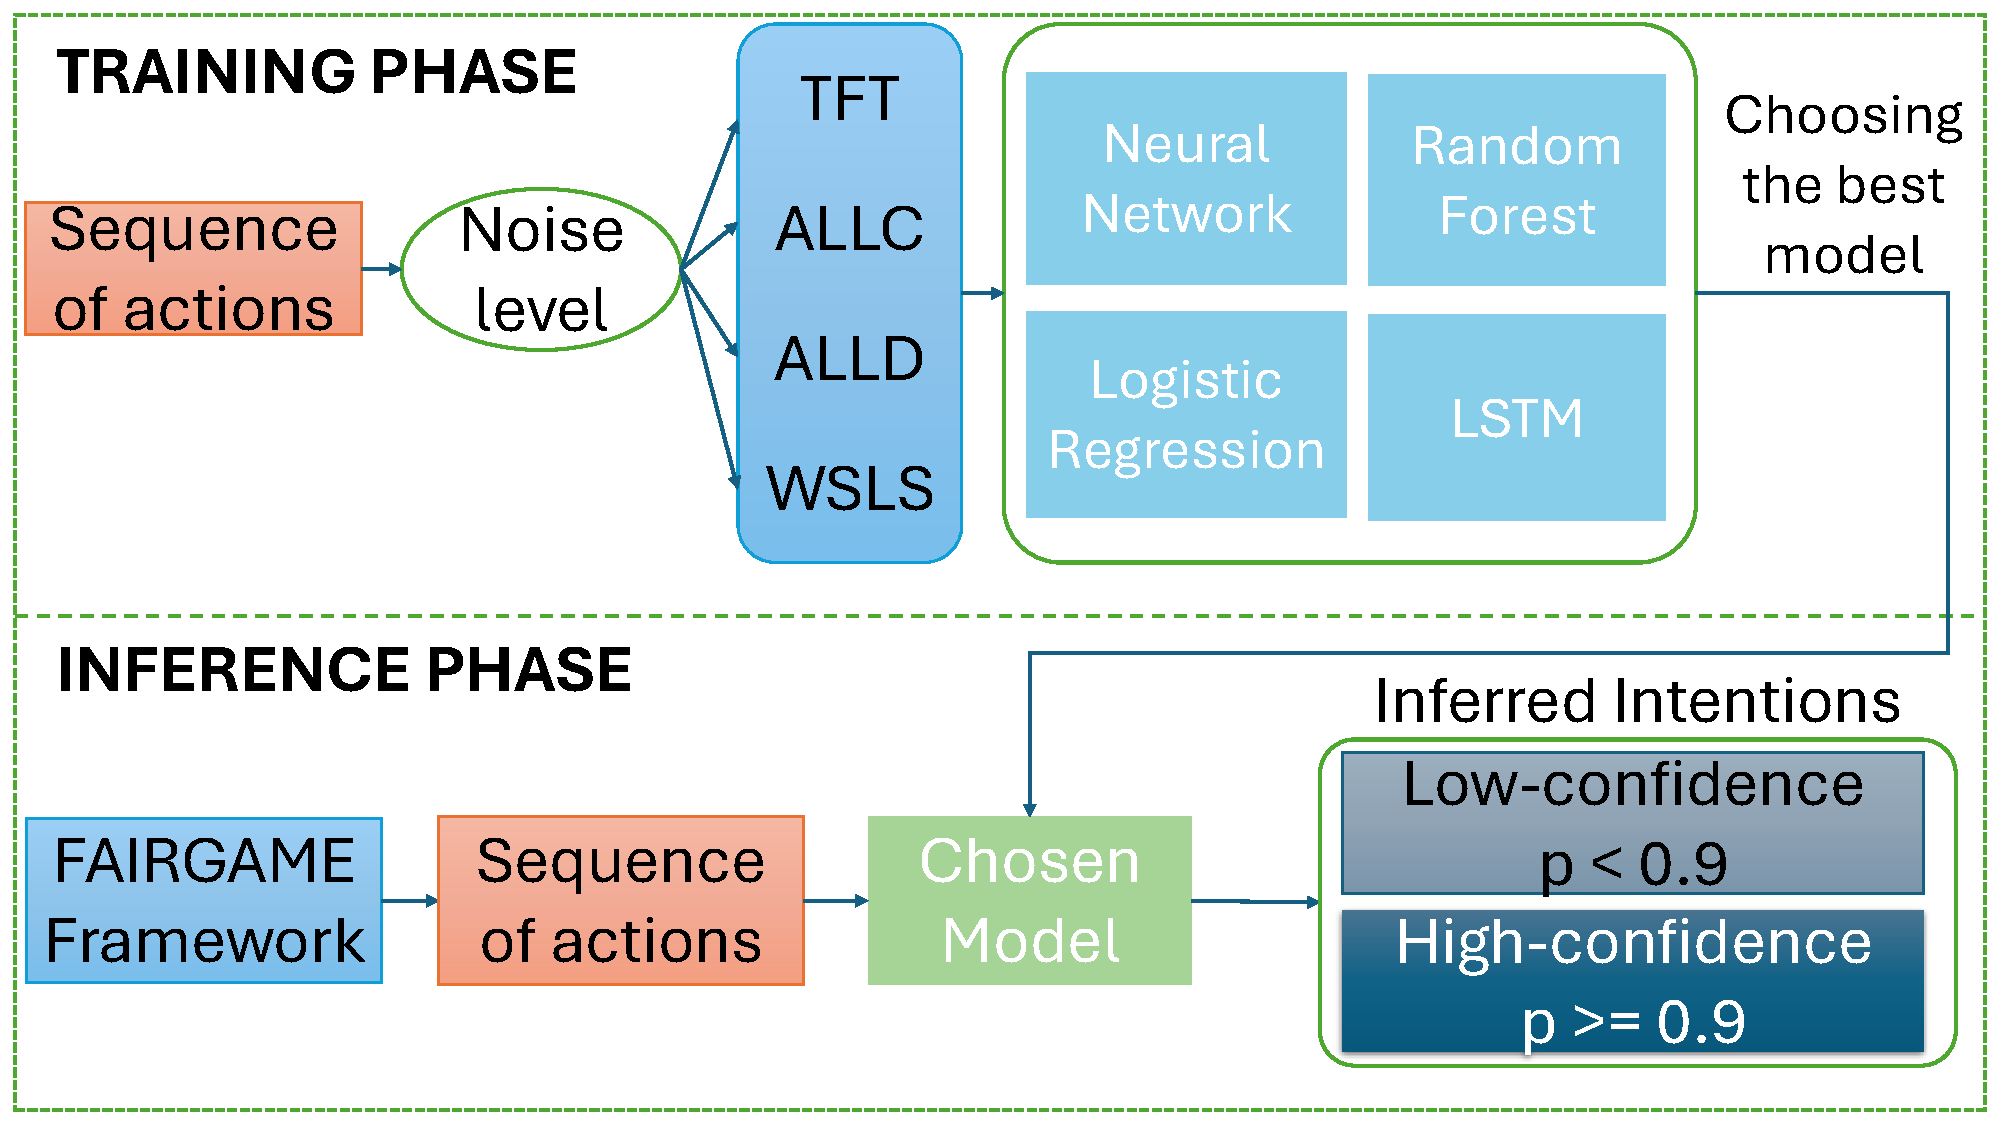
\includegraphics[width=0.6\linewidth]{all_figures/ijcai_fig9_intention_recognition_pipeline.pdf}
    \caption{Supervised learning pipeline for understanding LLM behaviour. Starting from action sequences associated with canonical strategies (ALLC, ALLD, TFT, WSLS) under varying noise conditions, we train supervised learning models to infer and classify underlying behavioural intentions. We then apply the best-performing model to the LLM repeated-gameplay data generated by FAIRGAME. High-confidence predictions ($>0.9$) are used to identify which strategies the LLM adopts, whereas low-confidence cases are reserved for subsequent analysis to investigate the possibility of emerging behaviours by the LLM.}
    \label{fig:supervised_intention_model}
\end{figure}

Following~\cite{diStefanoIntention2023}, we generate $10{,}000$ synthetic trajectories ($2{,}500$ per strategy, balanced) for four canonical strategies: TFT, ALLC, ALLD, and WSLS~\cite{sigmund:2010bo} (see Appendix~\ref{appendix:rule_based} for formal definitions). Each trajectory spans 10 rounds against a random opponent, with execution noise ($\epsilon \in \{0, 0.05\}$) injected to simulate LLM stochasticity. We train Logistic Regression~\cite{cox1958regression}, Random Forests~\cite{rf}, feed-forward Neural Networks~\cite{nn}, and Long Short-Term Memory (LSTM) recurrent networks~\cite{lstm} as candidate classifiers, selecting the best-performing model -- the LSTM -- for downstream inference because it can exploit the sequential structure of the action history. The choice matters: a static classifier treats each round in isolation, whereas a recurrent network can ``remember'' that the agent has, say, just been double-crossed three times in a row, which is exactly the kind of information a canonical conditional strategy uses.

FAIRGAME logs are preprocessed into state-action sequences encoding interaction outcomes: Reward ($R$), Punishment ($P$), Temptation ($T$), and Sucker ($S$). The trained model outputs probability distributions over strategy classes; we focus on high-confidence predictions ($>0.9$) to ensure reliability.


\section{Results}\label{sec:results}


\subsection{Payoff magnitude sensitivity}\label{sec:payoff_magnitude}

The results in this subsection are based on the payoff-scaled Prisoner's Dilemma experiments described in Section~\ref{sec:gameImportance}. These experiments evaluate three LLM models (GPT-4o, Claude~3.5~Haiku, and Mistral~Large) across five languages (Arabic, Chinese, English, French, and Vietnamese) under three payoff scaling conditions ($\lambda \in \{0.1, 1.0, 10.0\}$). Following the FAIRGAME framework~\cite{buscemi2025fairgame}, the payoff matrix represents \emph{penalties} (years of imprisonment in the Prisoner's Dilemma narrative), where lower values indicate better outcomes for agents. The agents' objective is to \emph{minimise} their cumulative penalties over the course of the repeated game.

Figure~\ref{fig:total_penalties} summarises the cooperative behaviour of the three proprietary LLMs across the payoff sweep. The two panels report the \emph{cooperation rate} -- the percentage of rounds in which an agent picked Option~B (cooperate) -- as a function of the stake multiplier $\lambda$, broken down (a) by model and (b) by prompt language. Lines are means across all games for a given cell; error bars are standard errors over games. The detailed per-(language, pairing, model) penalty grid that this figure summarises is reported in Appendix~\ref{appendix:proprietary_per_condition} for completeness.

\begin{figure}[!htbp]
    \centering
    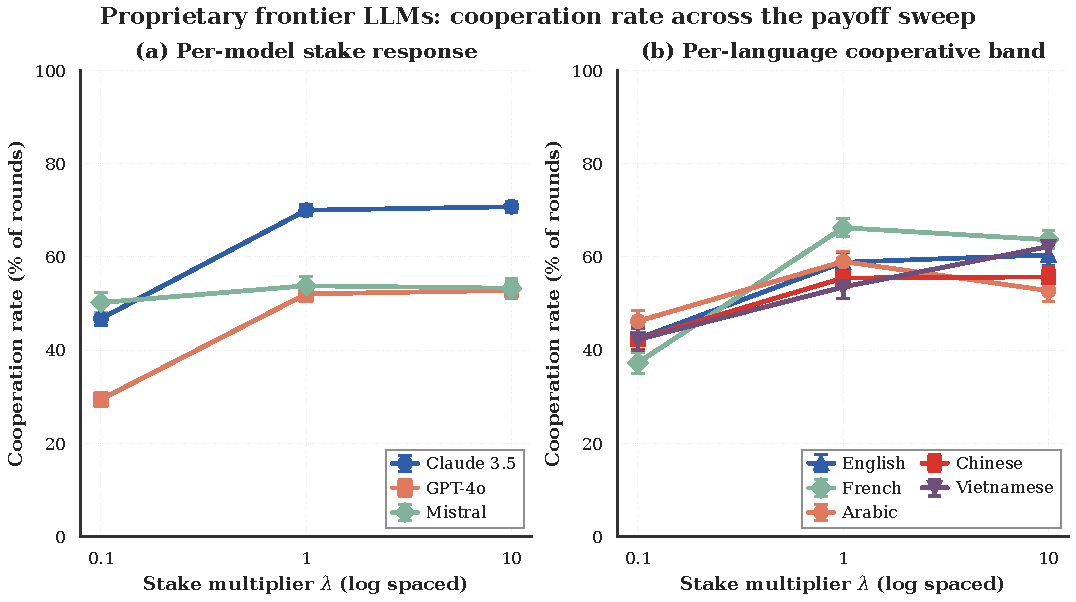
\includegraphics[width=0.85\linewidth]{all_figures/fig_proprietary_cooperation_overview.pdf}
    \caption{Proprietary frontier LLMs across the payoff sweep. The cooperation rate is the percentage of rounds in which an agent picked Option~B (cooperate); higher is more cooperative. \textbf{(a)} Per-model view: each model has a distinct stake response -- Claude~3.5 climbs steeply from low to moderate stakes and plateaus; GPT-4o shows the largest low-stake defection gap before recovering; Mistral Large is comparatively stake-insensitive. \textbf{(b)} Per-language view: French shows the largest stake-driven swing in cooperation, while Vietnamese rises monotonically across the sweep; Arabic and Chinese sit in similar mid-range bands.}
    \label{fig:total_penalties}
\end{figure}

The figure tells a short story. First, stake matters: every model and every language shows a higher cooperation rate at $\lambda \in \{1, 10\}$ than at $\lambda = 0.1$. Second, the response is model-specific. Claude lifts roughly twenty-five percentage points of its mass from defection to cooperation as stakes rise, GPT-4o starts from the lowest baseline and shifts the most absolutely, and Mistral Large barely moves at all. Third, the language axis carries comparable signal: French elicits the widest cooperative swing across stakes, while Vietnamese rises steadily into the highest band at $\lambda = 10$. The aggregate picture is consistent with the game-theoretic intuition that low stakes encourage exploratory defection while higher stakes commit agents to mutually beneficial play~\cite{han_when_2021}, but the model-level heterogeneity already hints that there is more going on than the payoff matrix alone explains. The subsections below decompose this picture in terms of inferred strategies and contrast it with the analytical evolutionary baseline.

Figure~\ref{fig:po_sensitivity_results} presents round-by-round choice trajectories. Claude~3.5~Haiku learns to cooperate over time, with attenuated-stake trajectories favouring defection. GPT-4o exhibits the opposite trend, converting to more defective behaviour over time, especially for the higher payoff stakes. Mistral~Large shows a different trend, with amplified payoffs correlating with increased defection - consistent with dominant strategy reasoning. A notable spike at Round~2 in Mistral's trajectories suggests retaliatory or probing behaviour~\cite{akata2025}.

Our additional analysis (Appendix~\ref{appendix:per_multiplier_metrics}, Figure~\ref{fig:per_multiplier_radar}) reveals that varying payoff stakes strongly impact LLM behavioural characteristics~\cite{buscemi2025fairgame}, particularly their internal variability (the variance of outcomes when the same game scenario is played multiple times).

\begin{figure}[!htbp]
    \centering
    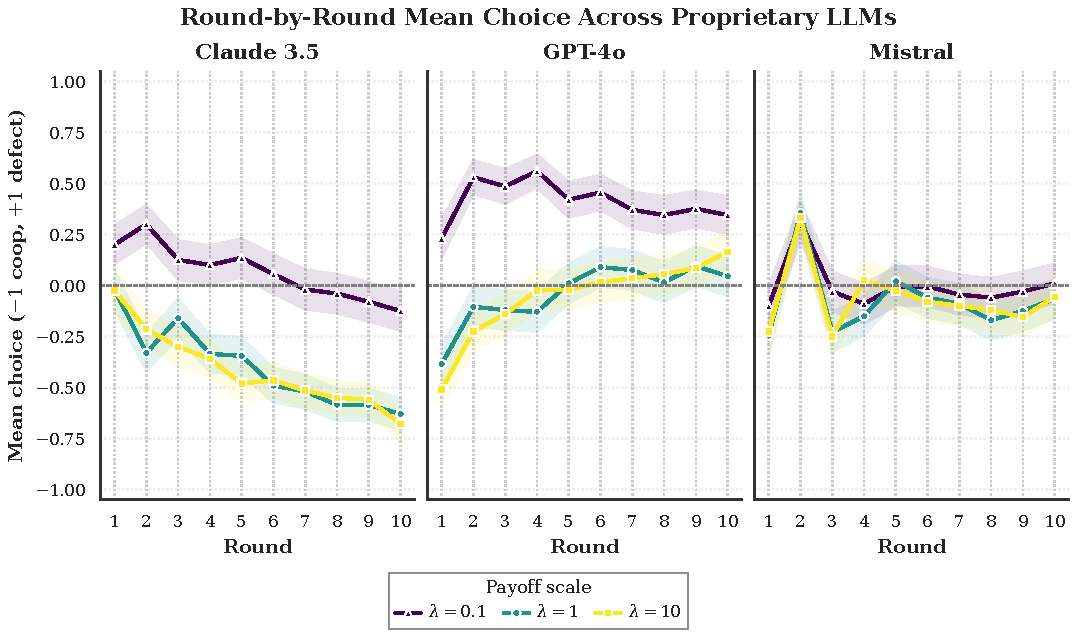
\includegraphics[width=0.9\linewidth]{all_figures/fig_large_trajectories.pdf}
    \caption{Average trajectory of strategy choices across repeated rounds in all Prisoner's Dilemma experiments, shown for each proprietary LLM (Claude~3.5~Haiku, GPT-4o, Mistral~Large) under different payoff magnitudes. A value of $+1$ indicates selection of Option A (defection), while $-1$ corresponds to Option B (cooperation); shaded bands denote standard errors across games. The experiments consider $\lambda \in \{0.1, 1.0, 10.0\}$, representing attenuated, baseline, and amplified penalty scales (viridis colour scale from dark purple to yellow). The three panels make the model-specific stake response visible: Claude~3.5 drifts towards cooperation across the horizon at $\lambda \in \{1, 10\}$, with amplified stakes reaching the most cooperative regime by round~10, while attenuated stakes ($\lambda{=}0.1$) keep it on the defection side throughout; GPT-4o starts cooperative at $\lambda \in \{1, 10\}$ but drifts steadily towards defection over rounds (consistent with end-game backward-induction reasoning); Mistral~Large shows a sharp Round~2 retaliatory spike before settling near the indifference line.}
    \label{fig:po_sensitivity_results}
\end{figure}

\subsection{LLM strategies in repeated games}\label{sec:llm_strategies}

We apply the intent recognition framework (see Section~\ref{subsec:intention_recognition}) to LLM decision trajectories to examine how their inferred strategic intentions vary with incentive magnitude, linguistic context, and model architecture. Before applying the classifier to unknown LLM trajectories, we validate it against synthetic baselines so we can distinguish genuine strategic shifts from classification artefacts. The LSTM classifier achieves $\text{F1} = 0.984$ on the 4-strategy task at $5\%$ execution noise and remains robust as the strategy space expands, successfully distinguishing behaviourally similar conditional strategies (Tit-for-Tat and Win-Stay--Lose-Shift)~\cite{sigmund:2010bo,diStefanoIntention2023}. It also outperforms Logistic Regression, Random Forest, and Hidden Markov Model baselines; the full benchmarking is reported in Appendix~\ref{appendix:robustness_noise}. Detailed strategy-recognition results on the baseline FAIRGAME corpus (four proprietary models at the default $\lambda{=}1$ condition) are provided in Appendix~\ref{appendix:baseline_fairgame}, including a complementary language-level analysis of agent scores and inferred strategies (Appendix~\ref{appendix:ml}).

We use a hybrid classification pipeline combining rule-based pattern matching for unambiguous trajectories with LSTM predictions for complex cases. Of the $3{,}600$ agent trajectories ($2$ agents $\times$ $1{,}800$ games), $2{,}914$ (approximately $81\%$) achieved classification confidence $\geq 0.9$ and were retained for analysis. Details on threshold sensitivity are provided in Appendix~\ref{appendix:threshold_sensitivity}; the rationale for selecting $\tau = 0.9$ as the primary cutoff is in Appendix~\ref{appendix:filtering_rationale}.

\paragraph{Mixed strategies within a trajectory.} A single-label assignment risks compressing trajectories that exhibit mid-game strategy switches into the nearest canonical archetype. We probe this in two complementary ways. First, our hybrid pipeline retains \emph{composite} labels of the form ``ALLD$|$TFT'' or ``ALLC$|$TFT$|$WSLS'' whenever a trajectory simultaneously satisfies the rule-based definition of more than one canonical strategy. Roughly one in four of the high-confidence trajectories receive such a composite label (see Appendix~\ref{appendix:mixture_labels} for the per-pattern breakdown). Second, we fit a four-state Hidden Markov Model whose hidden states correspond to the four canonical strategies and run Viterbi decoding on every trajectory (Appendix~\ref{appendix:hmm_segmentation}): the fraction of trajectories whose Viterbi path visits more than one hidden state is $20\%$, of the same order as the rule-based composite-label rate, and the average number of regime switches per trajectory is small (about 0.21 switches per trajectory on average). Crucially, re-aggregating the strategy distribution by redistributing each trajectory's mass over its visited HMM states preserves the directional stake effect documented in Section~\ref{sec:llm_strategies}: ALLD share still falls sharply between $\lambda{=}0.1$ and $\lambda{=}1$, and ALLC share still rises. We read this as evidence that within-trajectory mixing is real but moderate at the $N{=}10$ horizon, and that the single-label conclusions are conservative rather than overstated.

Figure~\ref{fig:strategy_trends_payoff} shows how strategy distributions shift with payoff scaling. As $\lambda$ increases from $0.1$ to $10$, we observe a clear behavioural inversion: unconditional defection (ALLD) sharply declines, effectively halving its prevalence, while conditional cooperation (WSLS) and unconditional cooperation (ALLC) both see marked increases. Tit-for-Tat (TFT) remains relatively stable across conditions. This aligns with standard stake-effect predictions and indicates that LLM agents are not statically aligned: they modulate their strategic commitments with incentive salience, transitioning from opportunistic defection at low stakes toward adaptive reciprocity (WSLS) as the consequences of error become more severe~\cite{han_when_2021,sigmund:2010bo}.

\begin{figure}[!htbp]
    \centering
    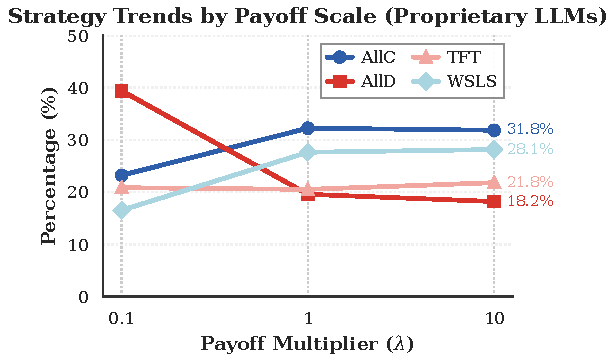
\includegraphics[width=0.58\linewidth]{all_figures/fig02_strategy_trends_by_lambda.pdf}
    \caption{Trends in inferred strategy distributions as a function of the payoff scaling parameter $\lambda$. Increasing payoff magnitude systematically shifts LLM behaviour from unconditional defection (ALLD) toward conditional and cooperative strategies (WSLS, ALLC), indicating sensitivity to incentive scale.}
    \label{fig:strategy_trends_payoff}
\end{figure}

Table~\ref{tab:strategy_by_llm} shows the aggregate and model-specific strategy distributions across all experimental conditions. Three patterns emerge. First, conditional strategies (WSLS and TFT) account for nearly half of all trajectories, almost matching unconditional strategies. This contrasts with game theory, which predicts universal defection in finite-horizon games via backward induction~\cite{sigmund:2010bo,Axelrod1980Effective}. LLMs instead use heuristics that respond to recent history, similar to bounded rationality in human players~\cite{akata2025,Han2012ALIFEjournal,lu2024llms}. Second, a moderate cooperative bias is evident: ALLC is more frequent than ALLD, consistent across payoff scales, languages, and models. This likely reflects alignment training, such as Reinforcement Learning from Human Feedback (RLHF) and Constitutional AI, optimising for prosocial behaviour~\cite{ouyang2022training,anthropic2022constitutional,buscemi2025strategic}. Third, strategic heterogeneity is high: distribution entropy approaches the theoretical maximum, indicating diverse strategic repertoires. This validates intent classification: aggregate cooperation rates alone would conflate fundamentally different decision rules~\cite{diStefanoIntention2023,Han2012ALIFEjournal}.

\begin{table}[!htbp]
\centering
\caption{Overall (aggregate) and model-specific strategy distributions in the payoff-scaled experiments (three models: Claude~3.5~Haiku, Mistral~Large and GPT-4o).}
\label{tab:strategy_by_llm}
\footnotesize
\begin{tabular}{lcccc}
\toprule
\textbf{Strategy} & \textbf{Overall} & \textbf{Claude} & \textbf{Mistral} & \textbf{GPT-4o} \\
\midrule
ALLC & 29.1\% & 29.7\% & 33.7\% & 23.7\% \\
ALLD & 25.9\% & 19.4\% & 25.2\% & 31.7\% \\
TFT  & 21.1\% & 25.1\% & 16.4\% & 22.8\% \\
WSLS & 24.0\% & 25.8\% & 24.8\% & 21.9\% \\
\bottomrule
\end{tabular}
\end{table}

Table~\ref{tab:strategy_by_llm} also shows model-specific strategy distributions. Claude~3.5~Haiku displays a cooperative strategic profile, with the highest level of overall cooperation (ALLC + WSLS + TFT), which is due to its highest level of conditional cooperation (WSLS + TFT). Mistral~Large shows the strongest unconditional cooperation bias, with ALLC being its most frequent strategy, though it retains diversity with ALLD and conditional behaviours. In contrast, GPT-4o exhibits a distinct ``hawk'' profile, with the highest defection rate. These differences persist across payoff scales and languages~\cite{buscemi2025fairgame,fontana2025nicer}, suggesting that training procedures and alignment methods imprint distinct strategic priors: some models are inherently ``dovish'' while others are ``hawkish.''

\begin{figure}[!htbp]
    \centering
    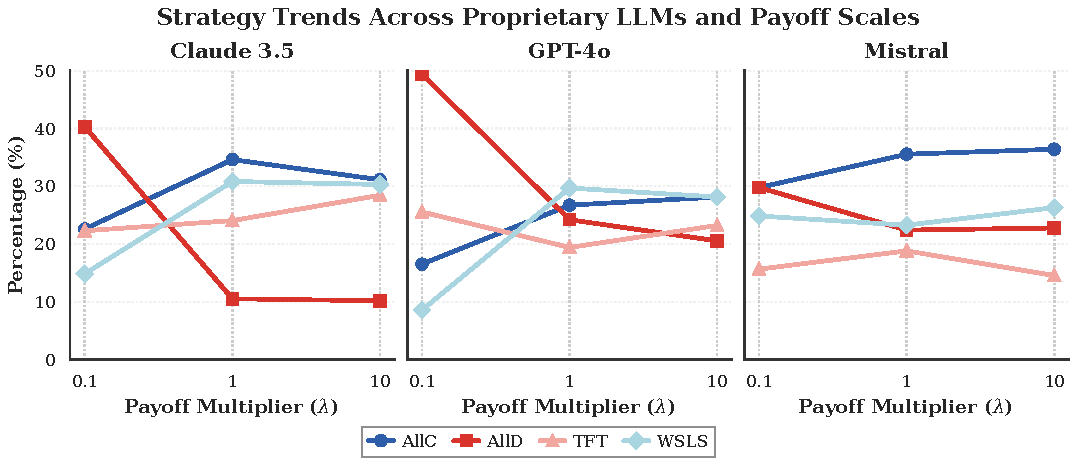
\includegraphics[width=0.9\linewidth]{all_figures/fig03_strategy_by_lambda_and_llm.pdf}
    \caption{Interaction between payoff scaling and LLM architecture. Each subplot illustrates how inferred strategies evolve with increasing payoff magnitude for a given model, revealing heterogeneous incentive sensitivity across LLMs.}
    \label{fig:payoff_llm_interaction}
\end{figure}

Crucially, Figure~\ref{fig:payoff_llm_interaction} shows that these priors interact non-trivially with payoff scaling, revealing \emph{architecture-dependent incentive sensitivity}. Across models, increasing $\lambda$ systematically shifts behaviour from unstable low-stake patterns toward stable strategies, though the extent of this shift varies by model. Claude and GPT-4o exhibit the highest payoff sensitivity: both models show steep reductions in ALLD prevalence as stakes move from attenuated to baseline levels, effectively abandoning widespread defection when consequences become non-trivial. GPT-4o is particularly responsive, shifting from a strongly defect-heavy regime at low stakes to a more balanced profile at baseline. Mistral Large, by contrast, demonstrates \emph{strategic inertia}: its ALLD rate varies by only a few percentage points across $\lambda$ values, whereas GPT-4o's ALLD share roughly halves between attenuated and amplified conditions (from $\approx 49\%$ at $\lambda = 0.1$ down to $\approx 21\%$ at $\lambda = 10$). This matches classical stake-effects where higher stakes amplify commitment to conventions, but highlights a critical nuance for AI governance: some models (like GPT-4o) are essentially rational agents that respond well to penalty tuning, while others (like Mistral) act as committed agents whose behaviour is stubbornly invariant to incentive design~\cite{fontana2025nicer}.

\begin{table}[!htbp]
\centering
\caption{Strategy distribution (\%) across languages, pooled over all $\lambda$ values. Arabic and Chinese exhibit the strongest bias toward unconditional strategies (ALLC+ALLD $\approx 60\%$), while English, French, and Vietnamese show more balanced distributions.}
\label{tab:language_strategy_distribution}
\footnotesize
\begin{tabular}{lccccc}
\toprule
\textbf{Strategy} & \textbf{Arabic} & \textbf{Chinese} & \textbf{Viet.} & \textbf{English} & \textbf{French} \\
\midrule
ALLC & 32\% & 32\% & 28\% & 28\% & 28\% \\
ALLD & 30\% & 28\% & 25\% & 22\% & 24\% \\
TFT  & 20\% & 18\% & 23\% & 23\% & 19\% \\
WSLS & 18\% & 22\% & 24\% & 27\% & 29\% \\
\bottomrule
\end{tabular}
\end{table}

A notable finding is the significant influence of linguistic context on strategic behaviour, an effect we term \emph{linguistic-cultural priming}. Table~\ref{tab:language_strategy_distribution} reveals that languages cluster into distinct strategic archetypes. Arabic and Chinese exhibit a shared bias toward unconditional strategies, with combined ALLC+ALLD around $60\%$. In contrast, English, French, and Vietnamese show more balanced profiles, with adaptive reciprocity (TFT+WSLS) and unconditional play roughly evenly split. English in particular displays the most uniform distribution across the four strategies, likely reflecting its dominance in training corpora~\cite{buscemi2025strategic}. An aggregated view grouping strategies into unconditional (ALLC\,+\,ALLD) vs.\ conditional (TFT\,+\,WSLS) classes is provided in Appendix~\ref{appendix:uncond_cond}.

\begin{figure}[!htbp]
    \centering
    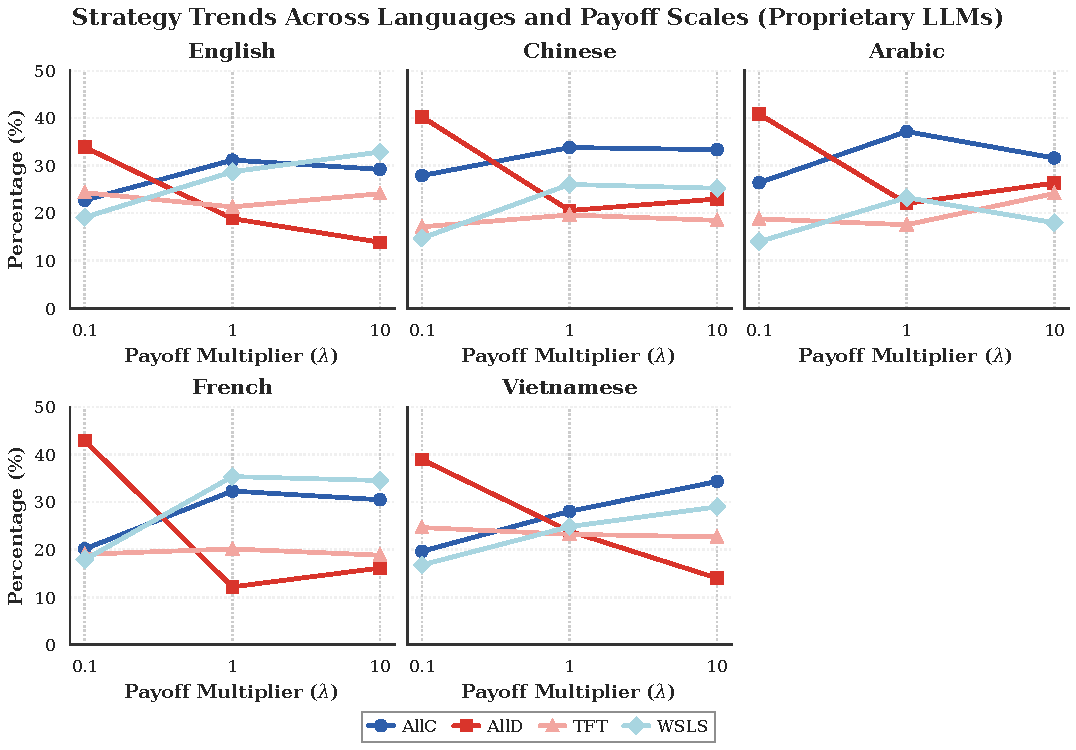
\includegraphics[width=0.9\linewidth]{all_figures/fig04_strategy_by_lambda_and_lang.pdf}
    \caption{Interaction between payoff scaling and language. Each subplot shows strategy evolution as $\lambda$ increases from $0.1$ to $10$. French and Vietnamese show the strongest stake-sensitivity, while Arabic exhibits the most muted response.}
    \label{fig:payoff_language_interaction}
\end{figure}

Moreover, these linguistic priming effects interact dynamically with incentive magnitude (Figure~\ref{fig:payoff_language_interaction}). All five languages start defection-oriented at low stakes but diverge sharply in how rapidly they shift toward cooperation as stakes rise. French and Vietnamese exhibit the strongest stake-sensitivity: French moves from the most defection-heavy profile at attenuated stakes to a WSLS-leading cooperative regime as stakes increase, while Vietnamese sees its cooperative share rise substantially over the same range. Arabic, by contrast, shows the most muted response, suggesting that some culturally-primed biases are more resistant to incentive pressure than others. Notably, at high stakes, English and French converge to nearly identical strategic profiles, suggesting that sufficiently strong incentives can normalise cross-linguistic variation. This has important implications for AI deployment: while language choice may introduce behavioural biases at low stakes, high-stakes environments may naturally mitigate some of these effects.

\FloatBarrier

\subsection{Statistical validation}\label{sec:statistical_validation}

To move beyond descriptive statistics, we conducted formal hypothesis testing using chi-square tests and factorial ANOVA (Table~\ref{tab:combined_validation}a). The results confirm that stake level significantly affects strategy distributions, and that different LLM architectures exhibit distinct incentive sensitivities. Post-hoc comparisons reveal the largest behavioural differences between attenuated and amplified stake conditions, with small-to-moderate effect sizes consistent with the inherent stochasticity of LLM decision-making~\cite{fontana2025nicer}. These statistical validations support our core finding: LLM strategic behaviour is systematically, i.e.\ not merely randomly, influenced by incentive design.

\begin{table}[!htbp]
\centering
\caption{Statistical validation summary: (a) hypothesis tests for stake effects, (b) classifier comparison for strategy recognition ($n=80{,}640$ test samples, 4-strategy, $5\%$ noise).}
\label{tab:combined_validation}
\footnotesize
\resizebox{0.6\linewidth}{!}{%
\begin{tabular}{lcccc}
\toprule
\multicolumn{5}{l}{\textbf{(a) Stake effect tests}} \\
\midrule
\textbf{Test} & \textbf{Statistic} & \textbf{p} & \textbf{Effect} & \textbf{Sig.} \\
\midrule
Chi-Square    & $\chi^2(6)=209.25$   & $<.001$ & $V=0.165$    & *** \\
1-Way ANOVA   & $F(2,3825)=48.25$    & $<.001$ & $\eta^2=0.025$ & *** \\
2-Way ANOVA   & $F(4,3823)=33.66$    & $<.001$ & $R^2=0.034$  & *** \\
\midrule
\multicolumn{5}{l}{\textbf{(b) Classifier performance}} \\
\midrule
\textbf{Model} & \textbf{Acc.} & \textbf{Prec.} & \textbf{Rec.} & \textbf{F1} \\
\midrule
LSTM              & \textbf{0.984} & \textbf{0.984} & \textbf{0.984} & \textbf{0.984} \\
Random Forest     & 0.980 & 0.980 & 0.980 & 0.980 \\
State-Factorised  & 0.956 & 0.958 & 0.956 & 0.956 \\
Neural Network    & 0.937 & 0.937 & 0.937 & 0.937 \\
HMM               & 0.777 & 0.826 & 0.777 & 0.780 \\
Logistic Reg.     & 0.756 & 0.767 & 0.756 & 0.751 \\
\bottomrule
\end{tabular}%
}
\end{table}

Our statistical tests treat trajectories as independent observations; however, the experimental design introduces nested dependencies: 10 repetitions per condition, 10 rounds per game, and 2 agents per game. For the chi-square test, the dependent variable is strategy category (4 levels); for ANOVA, we use a numeric encoding (ALLC$=1$, TFT$=2$, WSLS$=3$, ALLD$=4$) aggregated at the trajectory level. Mixed-effects multinomial logistic regression with random intercepts for repetition and game instance would better account for this nested structure and categorical outcomes; we acknowledge this as a methodological limitation. Our fixed-effects approach provides conservative estimates given consistent effect directions across conditions, and the threshold-sensitivity and label-expansion robustness checks reported in Appendices~\ref{appendix:threshold_sensitivity},~\ref{appendix:mixture_labels} and~\ref{appendix:hmm_segmentation} confirm the stability of our conclusions.

Deep learning models (LSTM, Neural Network) outperform probabilistic models (HMM, State-Factorised) on conditional strategies (TFT: LSTM $0.98$ vs HMM $0.74$; WSLS: LSTM $0.98$ vs HMM $0.73$), justifying our methodological choice. The State-Factorised model~\cite{fontana2025nicer} achieves $0.956$ accuracy, providing a strong SFEM-style baseline. While SFEM excels at estimating mixture proportions over long horizons (100+ rounds), our LSTM approach trades mixture flexibility for interpretable point estimates on shorter sequences.

The LSTM achieves near-perfect performance on unconditional strategies (ALLC/ALLD: F1 $=0.99$) but exhibits modest confusion between TFT and WSLS under noise, where execution errors can blur characteristic signatures. The Hidden Markov Model (HMM) baseline shows much higher confusion on conditional strategies (F1 $\approx 0.74$), justifying our LSTM choice. Confidence scores are uncalibrated; threshold sensitivity analysis (Appendix~\ref{appendix:threshold_sensitivity}) shows robustness across $\tau \in [0.7, 0.95]$.

\FloatBarrier

\subsection{Evolutionary game baseline: stationary strategy distributions under payoff scaling and execution noise}\label{sec:egt_baseline}

To complement the empirical analysis of LLM strategic preferences with a model-free theoretical benchmark, we computed the long-run frequency of the four canonical policies $\{$ALLC, ALLD, TFT, WSLS$\}$ predicted by evolutionary game theory (EGT) under the same payoff structure introduced in Section~\ref{sec:gameImportance}. The purpose of this analysis is twofold: (i) it characterises which strategy mixtures are evolutionarily stable when the only sources of variation are payoff magnitude and stochastic execution, and (ii) it provides a reference distribution against which the LLM-derived frequencies reported above can be directly contrasted. Combining EGT modelling with LLM-based simulations to interpret strategic divergences has recently proved fruitful in studies of AI governance dilemmas~\cite{balabanova2025media,buscemi2025llms}, and we adopt a similar logic here in the simpler payoff-scaled iterated Prisoner's Dilemma.

\paragraph{Model.} We adopt the standard pairwise-comparison process under the small-mutation limit (SML)~\cite{sigmund:2010bo,han_when_2021,nowak2004emergence,liu2020evolutionary}, in which a finite well-mixed population of size $Z = 100$ evolves through social imitation governed by the Fermi update rule. Small-mutation limit  here is a regime where mutations are rare enough that the population spends most of its time in monomorphic states (every individual playing the same strategy) and only occasionally transitions between them; this regime has a clean analytical solution and is the standard reference baseline in finite-population evolutionary game theory. This approximation has proven powerful in providing  predictions for human experimental data \cite{rand2013evolution,zisis2015generosity}. Selection intensity is set to $\beta = 0.1$ (weak-to-moderate selection) to suppress numerical overflow at large stakes while preserving the qualitative ordering of strategies. For each pair of resident strategy $i$ and mutant strategy $j$, the average per-round payoff $\pi_{ij}$ is computed analytically from a $r$-round iterated Prisoner's Dilemma. To ensure that the EGT analysis operates on the same incentive structure as the empirical experiments, we negate the FAIRGAME penalty matrix so that lower-is-better penalties in the empirical game become higher-is-better payoffs in the EGT calculation; this is a strict sign flip and preserves the strategic ordering of the dilemma. Concretely, the FAIRGAME penalties $T_{\text{pen}}{=}0$, $R_{\text{pen}}{=}2$, $P_{\text{pen}}{=}6$, $S_{\text{pen}}{=}10$ (representing years of imprisonment, so smaller is better) map to EGT payoffs $T{=}0$, $R{=}{-}2$, $P{=}{-}6$, $S{=}{-}10$ (so larger is better), and the standard Prisoner's Dilemma ordering $T > R > P > S$ is satisfied in both regimes. The whole matrix is then rescaled by the multiplier $\lambda$, identically to the empirical protocol of Section~\ref{sec:gameImportance}, so that the EGT and LLM comparisons are anchored to the same per-round incentive magnitudes. The fixation probability of a single $j$-mutant invading a resident $i$-population is
\begin{equation}
\rho_{ji} \;=\; \left(1 + \sum_{k=1}^{Z-1}\prod_{m=1}^{k}\frac{T^{-}_{ji}(m)}{T^{+}_{ji}(m)}\right)^{-1},
\end{equation}
where $T^{\pm}_{ji}(m)$ denote the Fermi-weighted up/down transition rates at composition $m$ \cite{szabo1998evolutionary}. Concatenating these probabilities yields an embedded Markov chain over the monomorphic states whose unique stationary distribution $\sigma$ encodes the long-run frequency of each strategy in the rare-mutation regime~\cite{sigmund:2010bo}. All quantities are obtained with the analytical pipeline of the open-source EGTtools library \cite{domingos2023egttools}, with the four canonical policies represented as memory-one strategies parameterised by an implementation-error rate $\varepsilon \in [0,1]$ that gives the per-round probability of executing the opposite of the intended action.

Figure~\ref{fig:egt_lambda_by_noise} show the EGT prediction into two complementary panels. The horizon is fixed at $r = 10$ rounds, matching the FAIRGAME experimental protocol \cite{buscemi2025fairgame}, and the population size and selection intensity are set as $Z = 100$, $\beta = 0.1$ throughout.

\begin{figure}[!htbp]
    \centering
    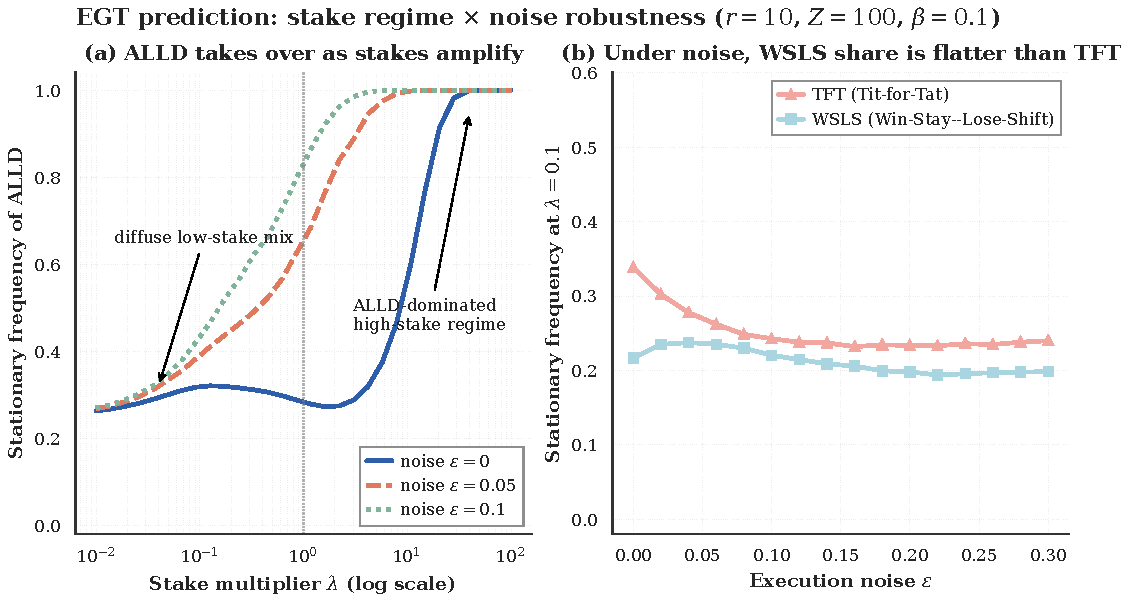
\includegraphics[width=\linewidth]{all_figures/fig10_egt_overview.pdf}
    \caption{\textbf{EGT prediction: stake regime $\times$ noise robustness ($r{=}10$, $Z{=}100$, $\beta{=}0.1$).} \textbf{(a)} Stationary frequency of Always Defect as a function of the stake multiplier $\lambda$ at three execution-noise levels. The Always-Defect line climbs from a diffuse low-stake mix to near-total dominance as stakes grow, and the three noise lines collapse onto one another in the high-stake regime: noise barely matters once stakes are amplified. \textbf{(b)} At low stakes ($\lambda = 0.1$), holding the stake fixed and varying execution noise $\varepsilon$, Tit-for-Tat remains the modal conditional cooperator but its frequency decreases monotonically as noise increases (from $\approx 34\%$ at $\varepsilon = 0$ to $\approx 24\%$ at $\varepsilon = 0.3$), while the Win-Stay--Lose-Shift frequency is  flatter ($\approx 22$--$26\%$ across the same range). It is important to note that a single execution error triggers a long sequence of retaliation between Tit-for-Tat players, whereas Win-Stay--Lose-Shift forgives its own mistakes automatically and so resists the noise pressure.}
    \label{fig:egt_lambda_by_noise}
\end{figure}

There are two notable observations. First, EGT predicts that high stakes should produce a wall of Always Defect, and the prediction is robust to execution noise: panel (a) shows the three noise curves converging to the same near-unity defection frequency for $\lambda \geq 10$. Second, the noise tolerance of the canonical conditional strategies is markedly asymmetric: panel (b) makes it visible at the stake level where conditional cooperators have any room to live at all. Both observations will feed directly into the comparison with the LLM data in the next subsection. The full per-strategy view at every stake and every noise level is reported in Appendix~\ref{appendix:egt_noise_sweep} as a more detailed reference.

\FloatBarrier

\subsection{Comparing EGT predictions and LLM-derived strategies}\label{sec:egt_vs_llm}

With the EGT prediction and the LLM data computed under matched conditions, we can finally ask the question that motivates this section: are LLMs playing the game as evolutionary theory expects them to play? Figure~\ref{fig:egt_vs_llm_bar} answers it visually. At low stakes the two distributions are not so far apart -- both lean defection-heavy, both leave some room for conditional cooperators. But as stakes grow the picture splits in two. The EGT bars collapse onto ALLD, as the classical theory says they should; the LLM bars do the opposite, drifting towards Win-Stay--Lose-Shift and unconditional cooperation. The same Prisoner's Dilemma, played by the same canonical strategies on the same payoff matrix, predicts two qualitatively different worlds depending on \emph{who} is playing -- EGT-style agents or LLM agents.

\begin{figure}[!htbp]
    \centering
    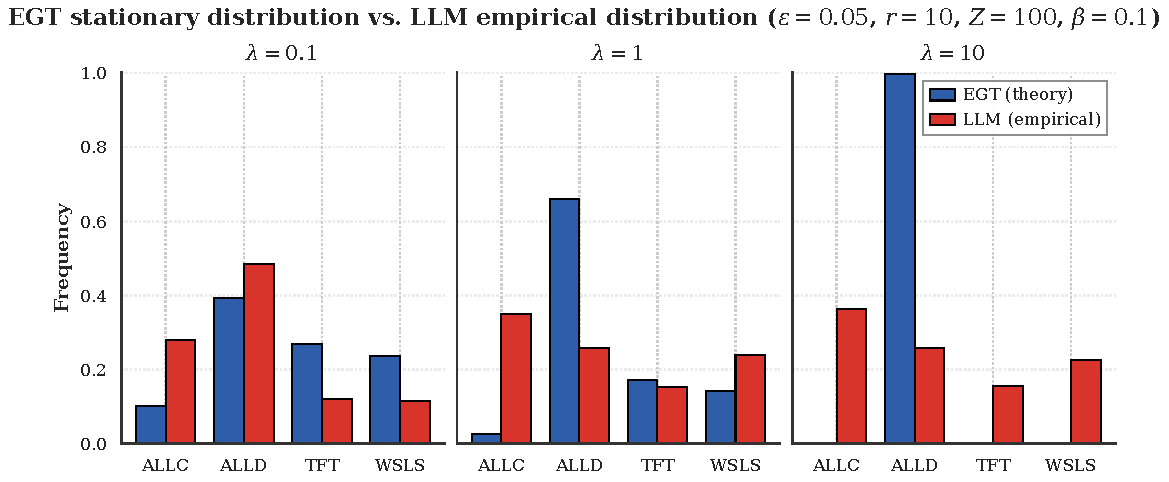
\includegraphics[width=\linewidth]{all_figures/fig19_egt_vs_llm_bar.pdf}
    \caption{\textbf{EGT stationary distribution (blue) vs.\ LLM empirical distribution (red) at $\lambda \in \{0.1, 1, 10\}$.} EGT computed analytically under the small-mutation limit with the FAIRGAME penalty matrix scaled by $\lambda$, $r{=}10$ rounds, $\varepsilon{=}0.05$ implementation noise, $Z{=}100$, $\beta{=}0.1$. LLM frequencies pool high-confidence ($\tau \geq 0.9$) trajectories of Claude~3.5~Haiku, GPT-4o, and Mistral~Large across all five languages at the matching $\lambda$, with composite (multi-rule) labels expanded into one row per matched canonical strategy so the distribution is consistent with Tables~\ref{tab:strategy_by_llm}--\ref{tab:language_strategy_distribution} and Figure~\ref{fig:strategy_trends_payoff}. At low stakes ($\lambda{=}0.1$) the two distributions agree on the ALLD-leading ranking but already disagree on the ALLC mass. As $\lambda$ rises, EGT concentrates virtually all mass on ALLD ($\approx 97\%$ at $\lambda{=}10$) while the LLM mix moves in the opposite direction, with ALLC and WSLS gaining share and ALLD declining to $\approx 18\%$.}
    \label{fig:egt_vs_llm_bar}
\end{figure}

\begin{table}[!htbp]
\centering
\caption{Pattern-by-pattern comparison of the EGT stationary distribution and the LLM empirical distribution at $r{=}10$, $\varepsilon{=}0.05$. Figure and table pointers embedded in the cells refer to the evidence reported elsewhere in this paper; numerical values in the ``EGT prediction'' column come from the analytical calculation reported in Section~\ref{sec:egt_baseline} and Figure~\ref{fig:egt_vs_llm_bar}, those in the ``LLM observation'' column come from Table~\ref{tab:strategy_by_llm} and Figure~\ref{fig:strategy_trends_payoff}.}
\label{tab:egt_vs_llm_summary}
\footnotesize
\begin{tabularx}{\linewidth}{XXX}
\toprule
\textbf{Pattern} & \textbf{EGT prediction} & \textbf{LLM observation} \\
\midrule
\multicolumn{3}{l}{\emph{Agreements}}\\
\midrule
Stake effect on strategy mix & $\lambda$ moves mass between conditional cooperators and ALLD & $\lambda$ shifts mass between ALLD and WSLS/ALLC \\
WSLS share is the most noise-stable conditional strategy & At $\lambda{=}0.1$, WSLS share holds within $\approx 22$--$26\%$ as $\varepsilon$ ranges over $[0, 0.3]$, while TFT share decays by $\approx 11$ percentage points (Fig.~\ref{fig:egt_lambda_by_noise}b) & WSLS share exceeds TFT in all three frontier models at $\lambda \in \{1, 10\}$ (gap of $\approx 2$--$12$~pp per model) \\
Highest behavioural diversity at low stakes & At $\lambda{=}0.1$, $\varepsilon{=}0.05$ all four canonical strategies retain non-trivial mass (ALLC $\approx 10\%$, TFT and WSLS $\approx 26\%$ each, ALLD $\approx 38\%$) & At $\lambda{=}0.1$ models maximally diverge in profile (Fig.~\ref{fig:payoff_llm_interaction}) \\
\midrule
\multicolumn{3}{l}{\emph{Divergences}}\\
\midrule
Direction of high-stake shift & ALLD concentration grows monotonically, reaching $\approx 97\%$ at $\lambda{=}10$ & ALLD share \emph{falls} from $\approx 39\%$ at $\lambda{=}0.1$ to $\approx 18\%$ at $\lambda{=}10$ \\
ALLC frequency & Near zero at $\lambda \gtrsim 1$ ($< 3\%$) & Persists at $23$--$32\%$ for every $\lambda \in \{0.1, 1, 10\}$ \\
Language dependence & Absent: EGT is language-blind & Strong (Table~\ref{tab:language_strategy_distribution}) \\
\bottomrule
\end{tabularx}
\end{table}

Table~\ref{tab:egt_vs_llm_summary} catalogues the agreements and divergences pattern by pattern. A chi-square test confirms what the eye already sees: the two distributions are statistically distinct at every stake we examined, and the gap between them \emph{widens} as $\lambda$ grows -- exactly the opposite of what would happen if LLMs were slowly converging to the rational equilibrium. The two systems are not drifting towards each other; they are pulling apart.

It is worth being clear about where the disagreement actually occurs. The two regimes do not always divert. They both pick up the existence of a stake effect: when consequences become larger, the strategy mix moves, on both sides. They both treat Win-Stay--Lose-Shift as the noise-stable conditional strategy: in the EGT prediction, the WSLS share is markedly flatter than the Tit-for-Tat share as execution noise rises (Fig.~\ref{fig:egt_lambda_by_noise}b), reflecting WSLS's self-correction from mutual defection \cite{imhof2007tit,han2011intention}; in the LLM data, the WSLS share exceeds the Tit-for-Tat share at $\lambda \in \{1, 10\}$ across our three frontier models. And they both place significant behavioural diversity at the low-stake end -- when little is at stake, both real and imagined populations can afford to explore. So far, EGT works as a useful first-order description of LLM strategic behaviour.

The disagreements are concentrated, and they are interpretive. The first is the direction of the high-stake shift. Theory says: when defecting is much more attractive, defection should win. LLMs say: when defecting hurts the partner that much more, defect less. The second is the existence of unconditional cooperation at all. With the same payoff structure, ALLC is strictly dominated and EGT eliminates it; LLMs always maintain a substantial level of ALLC across every stake level we tested. The third is language: the EGT baseline is, by construction, language-blind, while the LLM distribution varies  noticeably when the same game is re-prompted in Arabic, Chinese, English, French or Vietnamese.

It is tempting to read this as LLMs getting the game wrong. We think a more useful framing is that LLMs are playing a slightly different game, with three forces layered on top of the payoff matrix. The first is alignment training: RLHF and Constitutional AI~\cite{ouyang2022training,anthropic2022constitutional} reward prosocial completions, and that reward becomes most visible when penalties are strong, which is exactly the amplified-stake regime. The second is the human source of LLM training data: people in real repeated games tend to escalate cooperation, not defection, as the consequences of error grow~\cite{krockow2016cooperation,list2006friend}, and LLMs appear to have absorbed that pattern. The third is the prompt itself, which carries cultural connotations that evolutionary theory has no way of representing -- and so the EGT baseline cannot, by design, see the language effects we observe. In this way, the EGT baseline becomes useful precisely because it is naive: it tells us what the strategy mix would look like if payoffs and execution noise were the only forces in play, so that any systematic gap between EGT and LLM measures the contribution of the LLM-specific layers on top. This is the same logic that Balabanova~et~al.~\cite{balabanova2025media} arrived at in a governance setting -- and the consistency between their finding and ours is, in our view, the strongest single argument for treating EGT not as a competing predictor of LLM behaviour but as a normative reference against which LLM-specific biases can be diagnosed.

\FloatBarrier

\subsection{Open-weight small LLMs}\label{sec:small_llm}

A natural objection to everything reported so far is that proprietary frontier models share a narrow slice of the wider language-model landscape: they are large, aligned by similar Reinforcement Learning from Human Feedback (RLHF) pipelines, and trained on overlapping corpora. If our story is really about how language models behave as strategic agents -- and not about a specific generation of GPT and Claude -- the same patterns should hold when we step outside that slice. We therefore re-ran the payoff-scaled protocol on three open-weight small models that can be served locally on a single accelerator: Qwen3~8B~\cite{qwen3}, Gemma-3~12B~\cite{gemma3}, and Llama-3.1~8B~\cite{llama31}. The design follows Section~\ref{sec:gameImportance} exactly, with two extensions. First, the game horizon is extended from ten to thirty rounds, to ensure robustness of the previous consideration of ten rounds which might be  short for slow conditional strategies to surface can be put to rest. Second, the set of stakes is widened to six multipliers, $\lambda \in \{0.01,\, 0.1,\, 1,\, 10,\, 100,\, 1000\}$, spanning five orders of magnitude. Both extensions are deliberate: the wider range lets us look for any breakdown of the directional stake effect at extreme stakes, and the longer horizon lets us see whether late-game dynamics differ from the proprietary models. To match the extended game horizon, the LSTM component of the hybrid classifier was retrained on 30-round synthetic trajectories using the same architecture described in Section~\ref{subsec:intention_recognition}. A complementary classification on the first ten rounds is reported in Appendix~\ref{appendix:horizon_robustness} as a horizon-robustness check; it yields the same qualitative picture. In total, the open-weight replication covers $3 \text{ models} \times 5 \text{ languages} \times 6~\lambda \text{ values} \times 4 \text{ personality pairings} \times 10 \text{ repetitions} = 3{,}600$ games, yielding $216{,}000$ agent decisions (each game produces 60 decisions across $N{=}30$ rounds for 2 agents).

\begin{figure}[!htbp]
    \centering
    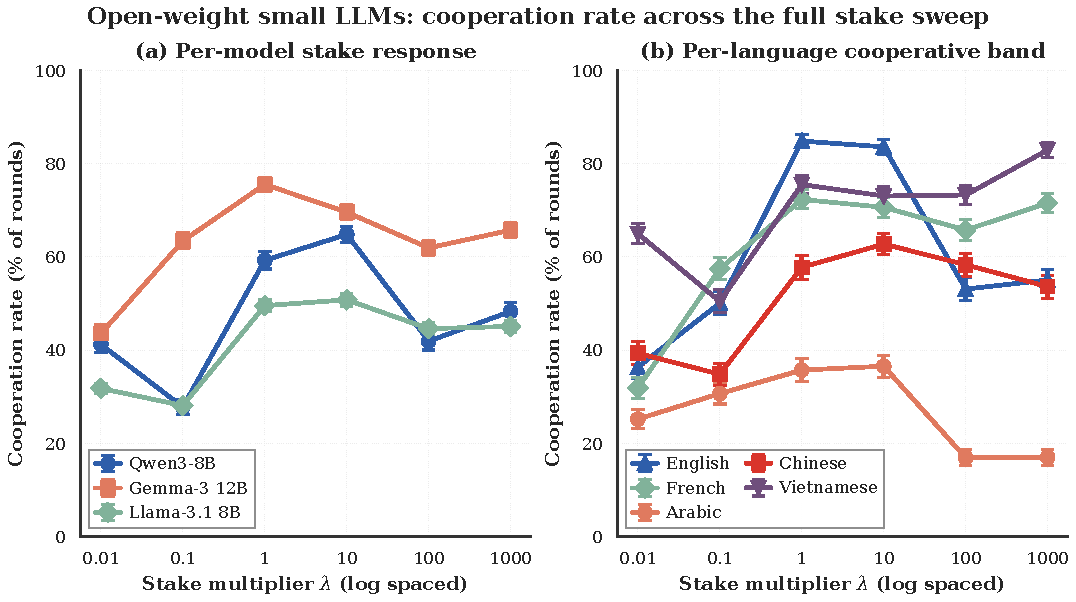
\includegraphics[width=\linewidth]{all_figures/fig_small_cooperation_overview.pdf}
    \caption{Open-weight small LLMs across the full stake sweep. Both panels show the cooperation rate -- the percentage of rounds in which an agent picked Option~B (cooperate) -- as a function of the stake multiplier $\lambda$ on a log-spaced axis. Error bars are standard errors over games. \textbf{(a)} Per-model view: each model has a different stake response. Gemma-3~12B occupies the highest cooperative band at almost every stake; Qwen3~8B traces a clear U-shape with its valley at the low-stake end; Llama-3.1~8B sits in the defection-leaning band, with a milder hump in the middle of the sweep. \textbf{(b)} Per-language view: each language occupies its own cooperative band. Vietnamese sits in the upper cooperative band across the sweep; Arabic the lowest; English shows the widest swing, peaking near $\lambda = 1$ and falling back at the very largest stakes.}
    \label{fig:small_cooperation_overview}
\end{figure}

There are three key observations, see  Figure~\ref{fig:small_cooperation_overview}. The directional stake effect of the main analysis is reproduced: cooperation rises as $\lambda$ grows out of the lowest cells. But it is not monotonic. At the very largest stakes, $\lambda \in \{100, 1000\}$, cooperation no longer keeps rising and in some cases drifts back down; the strongest version of this U-shape is Qwen3, whose cooperation rate climbs from roughly a quarter to roughly two-thirds and then partially relaxes. The middle of the sweep -- $\lambda \in \{1, 10\}$ -- is where cooperation is highest, suggesting that there is a particular range in stake magnitude that an EGT  would not predict at all. And the model identities matter: Gemma-3 inhabits the cooperative band across every stake, Llama-3.1 stays in the defection-leaning band, and Qwen3 occupies a context-sensitive middle zone. The proprietary observations about personality (cooperative pairings do better than selfish ones) and language (each model has its own cooperative language) remains  with the open-weight corpus. Further detailed per-(language, pairing) penalty breakdown is provided  in Appendix~\ref{appendix:small_per_condition_penalties}.

\begin{figure}[!htbp]
    \centering
    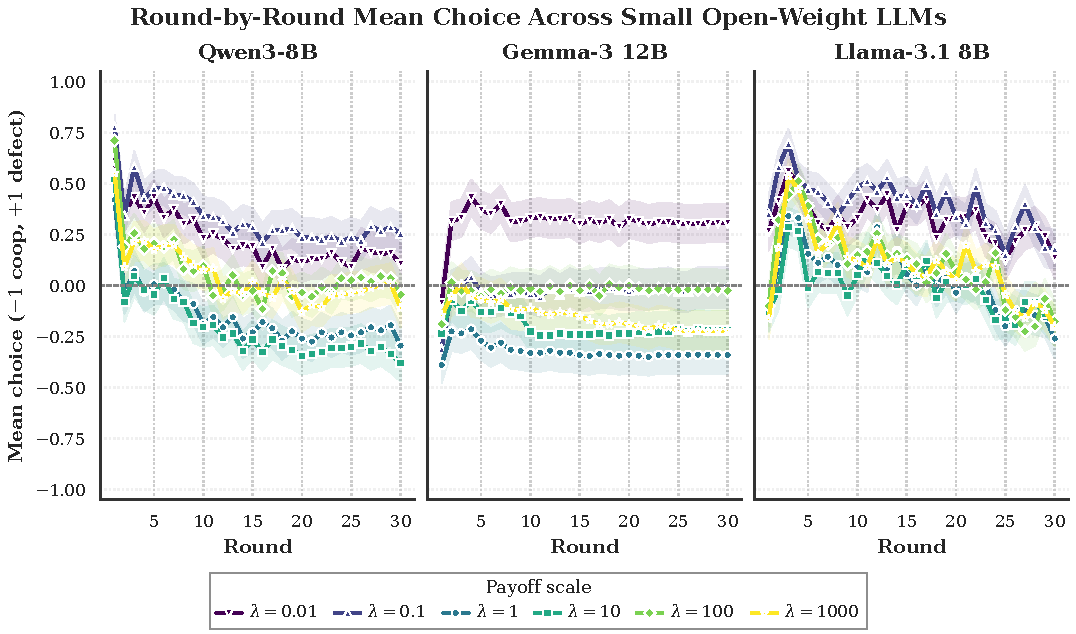
\includegraphics[width=\linewidth]{all_figures/fig_small_trajectories.pdf}
    \caption{Round-by-round mean choice trajectories for the three open-weight LLMs over the full $N{=}30$ rounds. The encoding ($+1$: defection; $-1$: cooperation) follows Figure~\ref{fig:po_sensitivity_results}. All three models shift towards cooperation as $\lambda$ rises. Qwen3~8B remains highly defective  throughout at $\lambda{=}0.1$ (mean choice $\approx +0.3$ to $+0.8$), while at $\lambda{=}\{1, 10\}$ it drifts steadily from a defection-leaning round~1 towards a cooperative regime by round~30 with no end-game defection spike. Gemma-3~12B is essentially stationary across rounds in every $\lambda$ condition. Llama-3.1~8B exhibits the largest stake-induced level shift in the mean-choice ($\pm1$) encoding: defection-heavy throughout at $\lambda{=}0.1$, mixed early oscillation at $\lambda{=}\{1, 10\}$ that gradually settles into a mildly cooperative regime by the final rounds.}
    \label{fig:small_trajectories}
\end{figure}

The round-by-round trajectories (Figure~\ref{fig:small_trajectories}) show the same story from a different angle. Gemma-3 commits to a policy in the first two rounds and then sticks to it, as a fixed-strategy player rather than a learner. Qwen3 keeps adjusting throughout the game, never fully settling, which fits its U-shaped stake response: a model that is constantly recalibrating to context is also a model that can be pushed in either direction by where the stake falls. Llama-3.1 keeps changing its behaviour  round-by-round but remains highly defective on average. None of the three open-weight models shows the late-game defection spike that backward induction would predict and that we observe in the proprietary trajectories: their cooperation, where it appears, persists to the last round. The most likely interpretation is that smaller models have shorter effective planning horizons and do not count down to the end of the game.

\begin{table}[!htbp]
\centering
\caption{Aggregate and per-model strategy distribution (\%) for the open-weight small LLMs ($N{=}30$ rounds, analysed with the hybrid intention-recognition pipeline of Section~\ref{subsec:intention_recognition}, with the LSTM component retrained on 30-round synthetic trajectories to match the extended game horizon). Shares are normalised over canonical strategy assignments at the $\tau{=}0.9$ confidence threshold; composite labels (e.g.\ ``TFT$|$WSLS'' when both strategies are matched) are expanded into one row per matched strategy before normalising.}
\label{tab:small_strategy_by_llm}
\footnotesize
\begin{tabular}{lcccc}
\toprule
\textbf{Strategy} & \textbf{Overall} & \textbf{Qwen3~8B} & \textbf{Gemma-3~12B} & \textbf{Llama-3.1~8B} \\
\midrule
ALLC & 20.74 & 21.19 & 21.60 & 17.46 \\
ALLD & 18.00 & 27.35 & 12.59 & 16.41 \\
TFT  & 41.98 & 35.55 & 40.85 & 57.00 \\
WSLS & 19.28 & 15.91 & 24.96 &  9.13 \\
\bottomrule
\end{tabular}
\end{table}

Table~\ref{tab:small_strategy_by_llm} shows the aggregate and per-model strategy distributions pooled over the extended stake range. Zooming in on which strategies underlie that cooperation reveals model-specific behavioural fingerprints (Figure~\ref{fig:small_strategy_by_model_lambda}). Gemma-3 stays balanced across the four canonical strategies at every stake, never letting any single mode dominate -- a kind of strategic generalist. Llama-3.1 does the opposite: at moderate stakes it collapses onto Tit-for-Tat, becoming the most committed reciprocator in the corpus, while at the extremes it tips back toward Always Defect. Qwen3 sits in between, with a U-shaped Always Defect curve whose valley is at the moderate stakes where the model is most cooperative. None of these patterns is what EGT would predict: the theory expects every model to walk uphill toward Always Defect as stakes grow, and only Llama-3.1 even partially follows that script.

\begin{figure}[!htbp]
    \centering
    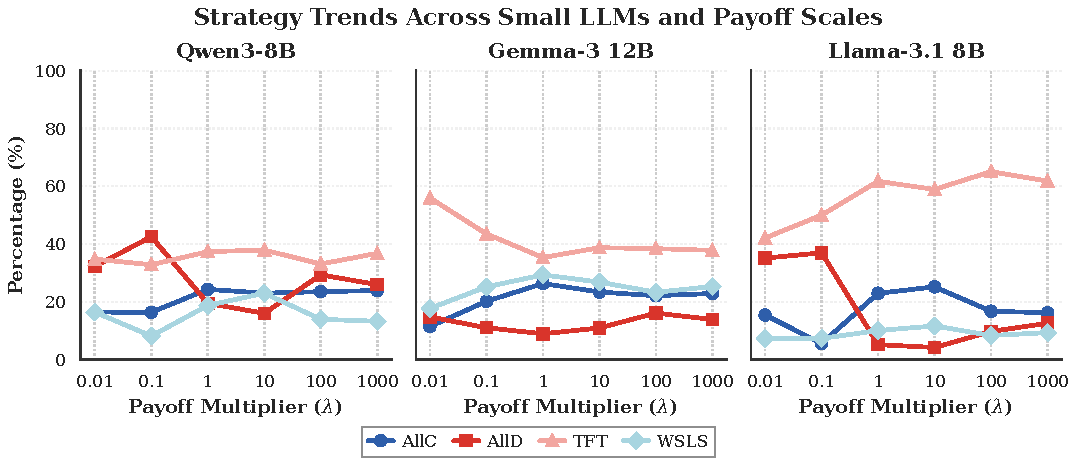
\includegraphics[width=\linewidth]{all_figures/fig17_multiplier_small_llm_interaction.pdf}
    \caption{Inferred strategy share for each open-weight LLM as a function of the payoff scaling parameter $\lambda$, normalised over canonical strategy assignments. The model-level interaction is heterogeneous: Gemma-3~12B remains comparatively low in ALLD ($9$--$16\%$) and balanced across the other three strategies at every stake; Llama-3.1~8B carries an elevated ALLD share at $\lambda \in \{0.01, 0.1\}$ but converges onto a strongly TFT-dominated profile (TFT $\approx 60\%$) from $\lambda = 1$ onward; and Qwen3~8B traces a U-shaped ALLD response, peaking at low stakes ($42.5\%$ at $\lambda = 0.1$) and again at very high stakes ($26$--$29\%$ at $\lambda \in \{100, 1000\}$), with a more balanced conditional mix in between.}
    \label{fig:small_strategy_by_model_lambda}
\end{figure}

\begin{table}[!htbp]
\centering
\caption{Strategy distribution (\%) across languages for the open-weight small LLMs (pooled over models and $\lambda$, normalised over canonical strategy assignments). Arabic is the most defection-heavy language, while Vietnamese has the largest TFT and WSLS shares and French has the highest ALLC share.}
\label{tab:small_strategy_by_language}
\footnotesize
\begin{tabular}{lccccc}
\toprule
\textbf{Strategy} & \textbf{Arabic} & \textbf{Chinese} & \textbf{Viet.} & \textbf{English} & \textbf{French} \\
\midrule
ALLC & 14.78 & 20.54 & 22.15 & 21.46 & 24.85 \\
ALLD & 33.92 & 17.73 &  9.61 & 14.54 & 14.17 \\
TFT  & 41.41 & 40.74 & 44.57 & 42.76 & 40.27 \\
WSLS &  9.89 & 20.99 & 23.67 & 21.24 & 20.71 \\
\bottomrule
\end{tabular}
\end{table}

The language story (Table~\ref{tab:small_strategy_by_language} and Figure~\ref{fig:small_strategy_by_language_lambda}) shows a similar trend: each prompt language sits in a different cooperative band, and the rank ordering survives the entire stake range. Vietnamese is the most reciprocity-oriented language, carrying the highest pooled Tit-for-Tat and Win-Stay--Lose-Shift shares and the lowest pooled Always Defect; the same ordering survives at the per-multiplier level for most, though not all, stakes. Arabic is the consistently defection-leaning language and the only one in which Win-Stay--Lose-Shift is essentially absent. English is the most stake-sensitive language, with cooperation rising sharply between the low and middle stakes and then easing back at the very largest stakes -- the U-shape we saw at the model level reappears here, sharpest on the English line of Figure~\ref{fig:small_cooperation_overview}b. French and Chinese fall between these extremes. The takeaway is that stake magnitude and prompt language interact: stake reshapes \emph{how much} cooperation a model produces, but the linguistic priors set \emph{which kind} of cooperation -- direct copy (Tit-for-Tat), self-correcting reciprocity (Win-Stay--Lose-Shift), or unconditional cooperation -- the model reaches for to produce it.

\begin{figure}[!htbp]
    \centering
    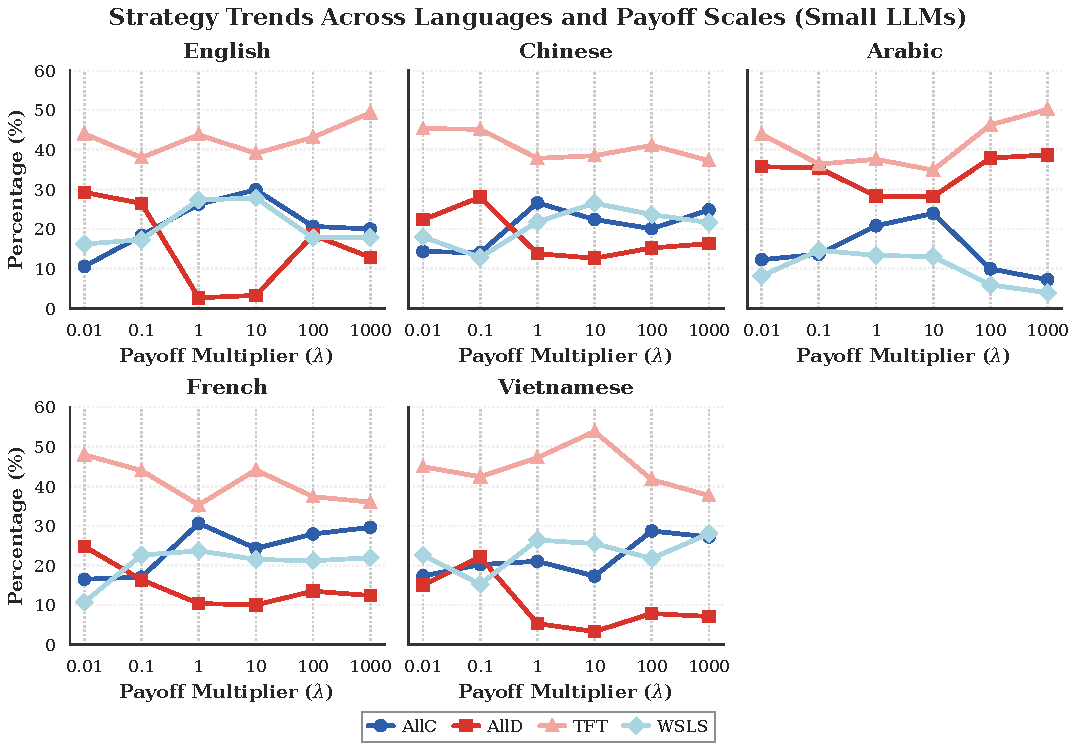
\includegraphics[width=\linewidth]{all_figures/fig18_multiplier_small_llm_language_interaction.pdf}
    \caption{Strategy share by language and payoff scaling for the open-weight LLMs (normalised over canonical strategy assignments). Arabic maintains the most defection-heavy profile across stakes; English exhibits the largest stake-driven retreat from ALLD (from $26$--$29\%$ at $\lambda \in \{0.01, 0.1\}$ down to under $4\%$ at $\lambda \in \{1, 10\}$). Vietnamese carries the highest TFT share at most stakes and a consistently elevated WSLS share; French carries the highest ALLC share at moderate stakes ($\lambda=1$) and at the largest stake ($\lambda=1000$), with Vietnamese or English topping the ALLC ranking at the intermediate stakes ($\lambda \in \{10, 100\}$).}
    \label{fig:small_strategy_by_language_lambda}
\end{figure}

The corresponding radar charts and three-way (language $\times$ model $\times$ game-stake) visualisations are reported in Appendix~\ref{appendix:per_multiplier_metrics} and Appendix~\ref{appendix:multidimensional} respectively, alongside the matched figures for the proprietary models so the two corpora can be inspected side by side. Additional robustness checks for the open-weight corpus -- including confidence-threshold sensitivity (Appendix~\ref{appendix:small_unfit}) -- are collected in Appendix~\ref{appendix:small_llm_robustness}.

Putting the two corpora side by side in Figure~\ref{fig:small_vs_main} provides a clear summary of what does and does not transfer between the proprietary and open-weight settings. What \emph{transfers} is the directional stake effect: in both groups, raising $\lambda$ out of the lowest cells pulls mass away from unconditional defection and toward conditional cooperation -- exactly the pattern that, in Section~\ref{sec:egt_vs_llm}, we argued is the most striking departure from the evolutionary baseline. The fact that this same signature reappears in a corpus of much smaller, openly released models that were not aligned by the same teams is, we argue, the strongest evidence we have that the divergence between evolutionary game theory and language models is a property of language models as a class, not an artefact of a particular vendor or generation. What does \emph{not} transfer is the texture of the cooperation. The proprietary corpus partitions itself roughly evenly across the four canonical strategies, while the open-weight corpus leans approximately two-to-one on Tit-for-Tat over Win-Stay--Lose-Shift (TFT $41\%$, WSLS $21\%$; ratio $\approx\!1.96$:$1$), which suggests that the smaller models implement reciprocity by copying the opponent's last action rather than by reading the joint outcome of the round. Whether this is a scale effect, a training-data effect, or a representational limitation of smaller models is an open question we leave for future work.

\begin{figure}[!htbp]
    \centering
    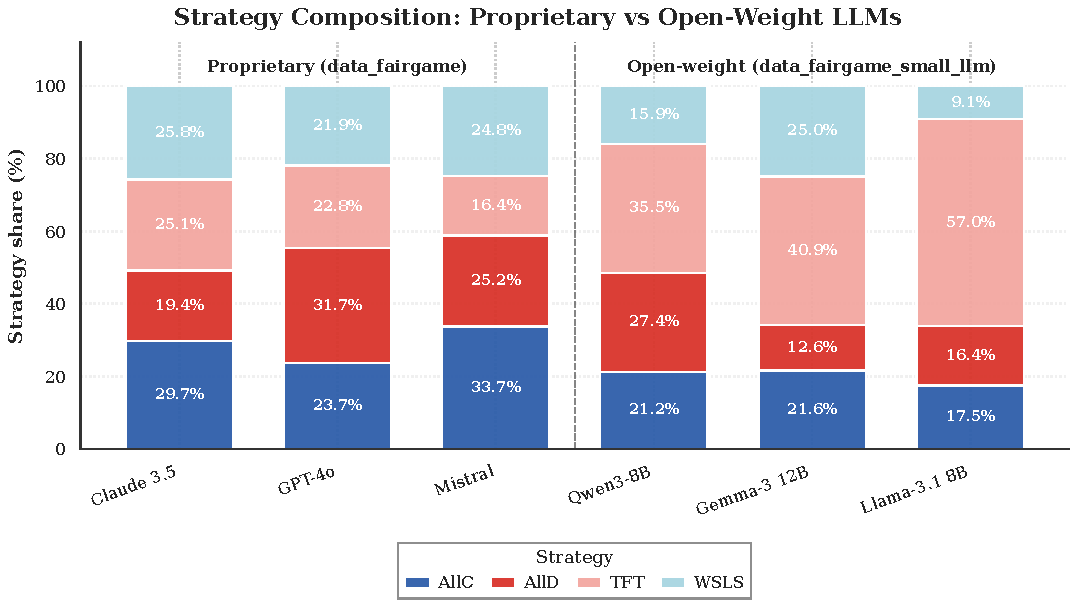
\includegraphics[width=\linewidth]{all_figures/fig_small_vs_main_strategies.pdf}
    \caption{\textbf{Strategy distribution: proprietary frontier models vs.\ open-weight small models.} Pooled high-confidence strategy frequencies of the three proprietary models (Claude~3.5~Haiku, GPT-4o, Mistral~Large at $N{=}10$ rounds) and the three open-weight small models (Qwen3~8B, Gemma-3~12B, Llama-3.1~8B at $N{=}30$ rounds) under the matched payoff-scaling design ($\lambda \in \{0.1, 1, 10\}$). The proprietary corpus partitions roughly evenly across the four canonical strategies (ALLC $29\%$, ALLD $26\%$, WSLS $24\%$, TFT $21\%$), whereas the open-weight corpus is TFT-dominated (TFT $41\%$, ALLC $22\%$, WSLS $21\%$, ALLD $16\%$). The directional stake effect is reproduced in both corpora; the open-weight corpus shows an approximately $2{:}1$ ratio of TFT to WSLS, consistent with a history-matching rather than outcome-conditioning style of reciprocity.}
    \label{fig:small_vs_main}
\end{figure}

A chi-square test on the high-confidence trajectories confirms that the dependence of strategy on stake is statistically significant in this corpus too, across all six stake values ($p$-values well below $10^{-20}$ for every model and below $10^{-49}$ for the pooled corpus; full per-model statistics in Appendix~\ref{appendix:small_llm_chi2}). The Cram\'er's $V$ effect sizes range from about $0.10$ for Gemma-3 (consistent with its stake-stable behaviour) to about $0.22$ for Llama-3.1 (consistent with its sharper between-stake collapse onto Tit-for-Tat at moderate $\lambda$).

Read together, these results give us three things. First, the headline pattern of the paper -- LLMs becoming more cooperative as stakes grow, in direct contradiction to the EGT prediction -- is not a frontier-model artefact. Second, the language and personality levers we identified for the proprietary models are at least as informative at the open-weight scale, and perhaps more so, since open-weight models have a wider behavioural range. Third, model identity still matters: each of the three open-weight models has a distinct strategic personality, from Gemma-3's balanced four-way mix, through Qwen3's U-shaped sensitivity to extreme payoffs, to Llama-3.1's committed Tit-for-Tat, and that personality coexists with the cross-cutting stake and language effects rather than overriding them. The diagnostic framework -- game-theoretic benchmarking, EGT baseline, supervised intent classification -- therefore generalises, and the cooperation biases it surfaces are not idiosyncratic to a small set of models. The conclusion is not driven by the longer horizon used for the open-weight runs either: an explicit check truncating each open-weight trajectory to its first ten rounds and re-classifying it (Appendix~\ref{appendix:horizon_robustness}) preserves both the agreement rate and the directional stake effect.

\FloatBarrier


\section{Discussion}\label{sec:discussion}


%If we step back from the figures, what does this paper actually claim?

We have shown that LLMs are sensitive to two control variables that are rarely considered  as control variables at all -- the size of the stakes of the interaction in place and the language of the prompt -- and that this sensitivity has a structure we can recover. Higher stakes pull LLMs towards reciprocal and cooperative behaviours; the language of the conversation among LLM agents pushes them towards either committed or adaptive strategies in patterns that correlate, loosely, with the cultural connotations of those languages in training data. Both effects are statistically confirmed in Section~\ref{sec:statistical_validation}. Neither lever is exotic, and neither is currently part of standard safety evaluations. Both shift behaviour by amounts that, in our data, rival the differences between model families.

Our central empirical claim -- that simply \emph{raising the stakes} of the underlying dilemma tilts LLMs towards cooperation -- is complementary to a parallel line of work that asks how external \emph{mechanisms} change LLM cooperation. CoopEval~\cite{tewolde2026coopeval} benchmarks contracts and mediation as cooperation-sustaining mechanisms; MoralSim~\cite{backmann2025moralsim} shows that moral framing modulates LLM cooperation in dilemmas where ethics and payoffs collide; cheap-talk pre-play communication has recently been shown to stabilise LLM strategic reasoning~\cite{loreheydari2026communication}. The reading we propose is that stake magnitude joins this list of cooperation levers: an intervention on the \emph{numerical} structure of the game, which sits alongside the linguistic and institutional interventions emphasised by these neighbouring lines of work.
Our findings thereby provide empirically grounded strategy profiles for LLM agents that can be directly integrated into models of evolutionary dynamics in hybrid human--AI populations, where artificial and human players co-evolve under shared incentive structures \cite{han2026social}.


The EGT comparison provides important and highly informative insights. Read literally, the comparison is a falsification result: evolutionary theory predicts that high stakes should produce result in high levels of defection, and LLMs produce the opposite. Read more usefully, it is a measurement: the gap between the EGT prediction and the LLM data is a quantitative signature of everything LLMs bring to the table that an evolutionary model does not -- alignment training, the cooperative bias of the human corpus, the cultural baggage of natural language. The fact that an independent EGT--LLM analysis of AI governance~\cite{balabanova2025media,buscemi2025llms} arrives at structurally similar mismatches -- LLM agents deviating from the rational equilibrium in the prosocial direction -- gives us some confidence that this is a real signal and not particular to our pipeline. Treating EGT as the null model and the LLM--EGT gap as the thing to be explained provides a productive way to read future studies of LLMs in strategic settings.

The open-weight replication shows the robustness of our findings for the frontier models (GPT and Claude). The same direction of stake effect, the same kind of language sensitivity, the same model-specific personalities all reappear at the $8$--$12$B scale. %, in a corpus of models that were not aligned by the same teams. 
The composition of the cooperation -- whether it is implemented through Tit-for-Tat or Win-Stay--Lose-Shift, whether it survives to the end of the game or collapses into late defection -- does change with scale, which is itself an interesting object for future work. But the high-level conclusion that LLMs are, for now, more cooperative than the underlying game-theoretic structure justifies appears to be robust across the scales we examined.

There are notable important implications for AI governance. Safety audits that run in English under fixed payoff conditions test a single point on a much larger behavioural surface. A model that is cooperative in English at moderate stakes can become measurably less cooperative in another language at low stakes, and the gap is not negligible. We would argue for adding two simple stress dimensions to existing evaluation suites -- a sweep over the stake of the underlying interaction, and a parallel run in the prompt's non-English variants -- and for anchoring the resulting measurements to an EGT baseline whenever the strategic structure permits it. This is what makes the difference between describing what an LLM \emph{does} and understanding what it is responding \emph{to}.

We conclude by noting several important caveats regarding the scope and limitations of our analysis. First, our intent classifier  is restricted to four canonical strategies, so  more complex strategy classes  such as Zero-Determinant play~\cite{pressDyson2012,hilbe2013memory}, mixed policies, extortionate strategies is mapped into the nearest canonical type. The hybrid rule pipeline does retain a \emph{composite} label whenever a trajectory satisfies more than one canonical rule, and roughly one in four high-confidence trajectories falls in that composite category (Appendix~\ref{appendix:mixture_labels}); re-attributing these trajectories under a uniform-mass tie-breaking rule shifts the aggregate frequencies by only a few percentage points and does not affect any qualitative conclusion. Nevertheless, the underlying single-label assumption constitutes a substantive modelling choice, and a mixture or segmentation model along the lines of SFEM~\cite{fontana2025nicer} or the probabilistic estimators of~\cite{inferenceStrategies} would be a natural next step. 

Second, the ten-round known-horizon setting we use with the proprietary models is conducive to backward-induction defection in the final rounds, and although the thirty-round runs with the open-weight models argue that this is not what drives the main stake effect, the question of whether the high-stake cooperation pattern survives an \emph{indefinite}-horizon condition is open and worth a follow-up. 

Third, our decoding settings follow each provider's recommended defaults: GPT-4o and Claude run at temperature $1.0$ while Mistral Large runs at $0.3$, and this difference cannot be cleanly separated from architectural effects in our data; a controlled ablation that fixes temperature and top-$p$ across models would tighten the causal story. 

Fourth, the EGT baseline maps LLM stochasticity onto a symmetric per-action flip probability $\varepsilon$, which is a clean theoretical object but a coarse abstraction of LLM variability: cognitive heuristics, prompt sensitivity, and end-game reasoning are not well captured by  symmetric flips. Accordingly, the EGT calibration we report should be treated as a reference distribution rather than a fitted model. An empirical estimation of an effective $\varepsilon$ from LLM self-play against deterministic opponents would tighten this link, and we leave it for future work. 

Fifth, our statistical tests treat trajectories as independent observations even though the design has nested dependencies (two agents per game, ten or thirty rounds per game, ten repetitions per condition); mixed-effects multinomial models with random intercepts for game and repetition would be more rigorous, and the effect sizes we report should be read as approximations. Finally, we have not benchmarked against human data on the same payoff matrix; that comparison, on which a separate literature exists~\cite{krockow2016cooperation,list2006friend}, is the next natural step.\\


In summary, language and incentives are not  implementation details but fundamental control variables, and the strategies that LLMs exhibit in repeated interactions are most appropriately understood as the joint outcome of these control variables, the underlying game structure, and the model-specific layers inferred from discrepancies between empirical behaviour and an evolutionary baseline.

%%%%%%%%%% End matter (Royal Society statements) %%%%%%%%%%

\ethics{This work did not involve human participants, animal subjects or fieldwork; all experiments are computational simulations of interactions between large language model agents.}

%% TODO(authors): insert the repository/DOI before submission.
\dataccess{The gameplay logs, prompt templates, trained classifiers and analysis code supporting this article will be made publicly available upon acceptance.}

%% TODO(authors): complete the CRediT-style contribution statement.
\aucontribute{T.-K.H. and D.-S.D.-M. contributed equally to this work and are joint first authors. All authors contributed to the research and the writing of the manuscript, and gave final approval for publication.}

\competing{The authors declare that they have no known competing financial interests or personal relationships that could have appeared to influence the work reported in this paper.}

\funding{T.A.H. is supported by EPSRC (grant EP/Y00857X/1).}

\ack{T.A.H. acknowledges travel support from the HCMUT-VNUHCM (Adjunct Professorship scheme HCMUT-VNUHCM).}

%%%%%%%%%% Bibliography %%%%%%%%%%

\printbibliography

\end{document}
